\documentclass{report}
\usepackage[utf8]{inputenc}
\usepackage[T1]{fontenc}
\usepackage[french]{babel}
\usepackage{amsmath}
\usepackage{amssymb,amsfonts,textcomp}
\usepackage{array}
\usepackage{hhline}
\usepackage{hyperref}
\hypersetup{colorlinks=true, linkcolor=blue, citecolor=blue, filecolor=blue, urlcolor=blue, pdftitle=, pdfauthor=Gilles Vuidel, pdfsubject=, pdfkeywords=}
\usepackage{graphicx}
\usepackage[top=2.501cm,bottom=2.501cm,left=2.501cm,right=2.501cm,nohead]{geometry}
\usepackage{float}
\usepackage{parskip}
\usepackage{multirow}
\usepackage{caption}
\usepackage{fancyvrb}
\makeatletter
\newcommand\arraybslash{\let\\\@arraycr}
\makeatother
% centering figures
\makeatletter
\g@addto@macro\@floatboxreset\centering
\makeatother
\setlength\tabcolsep{1mm}
\renewcommand\arraystretch{1.3}

% saut de page après une section
%\let\oldsection\section
%\renewcommand\section{\clearpage\oldsection}

% saut après itemize
\let\EndItemize\enditemize
\def\enditemize{\EndItemize\medskip}

\begin{document}
 \begin{titlepage}
	
	\centering
	
\includegraphics[scale=0.5]{img/logo.png}\\
	
	\bigskip
	\bigskip
	\bigskip	
	{\Huge
		\bfseries
		PixScape 1.1.5\\
		\bigskip
		Manuel d’utilisation\\
	}
	\bigskip
	\bigskip
	\bigskip
	\bigskip
	\bigskip
	
	{\Large		
		Gilles Vuidel, Yohan Sahraoui et Jean-Christophe Foltête\\
		\bigskip
		19/04/2019\\
	}
	
\end{titlepage}

\setcounter{tocdepth}{2}
%\renewcommand\contentsname{}
\tableofcontents

\pagebreak

\chapter{Introduction}

\section{A propos de PixScape}

Le logiciel PixScape est dédié à l'analyse du paysage visible à partir de données raster en 2D et demi. Il offre l’avantage d’être un outil intégré regroupant l’ensemble des fonctionnalités disponibles dans les outils SIG standards existants dans ce domaine et proposant d’autres fonctions originales comme la vue tangentielle et la gestion des données multi-résolution.


\subsection{Auteurs}
Le programme PixScape a été développé au laboratoire \href{http://thema.univ-fcomte.fr}{ThéMA} (\href{http://www.univ-fcomte.fr}{Université de Franche-Comté} – \href{http://www.cnrs.fr}{CNRS}) par Gilles Vuidel en collaboration avec Jean-Christophe Foltête, Daniel Joly, Yohan Sahraoui et Samy Youssoufi. Le logo a été réalisé par Xavier Girardet.

\subsection{Conditions d’utilisation}
Le programme PixScape est disponible librement sous licence \href{https://www.gnu.org/licenses/gpl-3.0.fr.html}{GPL}. Le code source est téléchargeable à partir du dépôt Git : \url{git://git.renater.fr/pixscape.git}.

Les utilisateurs de PixScape sont invités à citer la référence  suivantes  dans leurs travaux :

Sahraoui Y., Vuidel G., Foltête J-C. et Joly D. (2016), \href{http://cybergeo.revues.org/27862}{PixScape – un outil logiciel intégré pour l’analyse du paysage visible}, Cybergeo : European Journal of Geography, GeOpenMod - Modèles et logiciels, document 799. 


\section{Configuration requise}

PixScape fonctionne sur n'importe quel ordinateur supportant Java 7 ou supérieur (PC sous Linux, Windows, Mac...). Toutefois, lorsqu'il s'agit de données très volumineuses, la quantité de mémoire vive (RAM) de l’ordinateur peut limiter la taille des zones d'étude. De plus, la puissance du processeur va déterminer la vitesse de leur calcul. Vous trouverez plus de détails à ce sujet dans le chapitre \nameref{perf}. 

Pour l'utilisation de l'accélération GPU, l'ordinateur doit être équipé d'une carte graphique Nvidia supportant CUDA. Par défaut, PixScape est compilé avec la version 6.5 de CUDA. Si vous ne pouvez pas installer la version 6.5 de CUDA, il faudra installer la bibliothèque JCuda correspondant à votre version de CUDA et lancer le programme en ligne de commande (voir \nameref{cuda}). Les binaires sont téléchargeables à l'adresse \href{http://www.jcuda.org/downloads/downloads.html}{www.jcuda.org/downloads/downloads.html}

\section{Installation et lancement du programme}

PixScape est téléchargeable à cette adresse : \url{http://sourcesup.renater.fr/pixscape}.

\begin{itemize}
	\item Télécharger et installer Java 7 ou + (\href{http://www.java.com}{java.com}). Installer de préférence la version 64 bits de Java.
	\item Télécharger pixscape-1.1.jar
	\item Lancer pixscape-1.1.jar
\end{itemize}

PixScape peut être utilisé par deux interfaces : une interface graphique et une interface en ligne de commande.
L'interface graphique permet de créer un projet, visualiser les données, calculer de manière interactive les vues et les métriques, et de calculer de manière exhaustive les métriques de visibilité sur son ordinateur local. L'interface en ligne de commande permet quant à elle, de lancer ces même calculs sur des ordinateurs distants ainsi que sur des clusters.

Le chapitre suivant (\ref{gui}) décrit l'ensemble des fonctionnalités du logiciel disponibles à partir de l'interface graphique. Le chapitre \ref{cli} détaille comment utiliser PixScape en ligne de commande. Le chapitre \ref{principles} explique comment sont implémentés les calculs de visibilité dans PixScape. L'ensemble des métriques disponibles sont détaillées dans le chapitre \ref{metrics}. Et le chapitre \ref{perf} revient sur les modes de parallélisation, les performances et la gestion mémoire.




\chapter{Interface graphique}
\label{gui}

Une fois PixScape lancé, la première étape consiste à créer un projet basé sur un MNT (Modèle Numérique de Terrain) couvrant la zone à étudier.

\section{Création d'un projet}

La mise en place d’un nouveau projet PixScape s’effectue à partir du menu : Fichier / Nouveau projet. L’utilisateur doit renseigner un nom et un chemin pour le projet ainsi qu'un MNT au format Tiff ou AsciiGrid. \textbf{Le système de coordonnées du MNT doit obligatoirement être projeté et en unité métrique. Si ce n'est pas le cas, les calculs de visibilité seront erronés.} La résolution des altitudes (Z) peut être précisée si elle n'est pas métrique. Par exemple, si les altitudes sont données en centimètre, il faudra saisir 0.01 dans "Résolution Z".

\begin{figure}[H]
	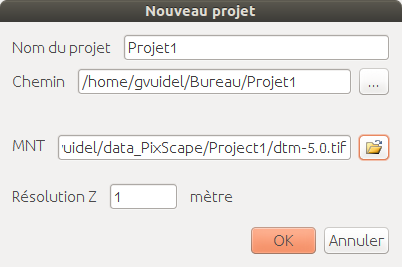
\includegraphics[scale=0.5]{img/new_project-fr.png} 
	\caption{Création d'un projet}
\end{figure}

Le projet créé stocke dans son dossier, le MNT transformé en Tiff avec les altitudes en résolution métrique ainsi qu'un fichier XML conservant les paramètres du projet.
Pour ouvrir un projet, il suffit de sélectionner le fichier XML correspondant à partir du menu Fichier / Charger un projet.

Dans PixScape, le MNT est suffisant pour réaliser des calculs de visibilité, mais il est souvent plus intéressant d'ajouter des informations complémentaires pour réaliser des analyses plus précises.

\section{Gestion des données}

Pour les données raster à importer, PixScape supporte deux formats de fichier : Tiff et AsciiGrid. Pour le format Tiff, le système de coordonnées peut être donné de deux manières : directement dans le fichier Tiff par l'extension GeoTiff ou bien par un fichier texte additionnel ayant le même nom et l'extension .tfw. 


\subsection{Couches complémentaires}
Deux couches raster complémentaires peuvent être ajoutées à un projet existant : le MNE (Modèle Numérique d'Élévation) et l'occupation du sol.

\subsubsection{MNE}
Le MNE correspond à la hauteur des objets (bâtiments, arbres, etc) au sol. L'addition du MNT et du MNE permet d'obtenir l'élévation totale des éléments du paysage. L'unité des hauteurs doit être obligatoirement exprimée en mètre. Pour charger un MNE, il suffit de sélectionner un fichier raster au format Tiff ou Asciigrid à partir du menu Données / Charger MNE. Après son chargement, le MNE est stocké dans le répertoire du projet.

\subsubsection{Occupation du sol}
La couche d'occupation du sol est utilisée par plusieurs métriques de configuration paysagère (S, IJI, CONTAG, etc). Les codes des catégories d'occupation du sol doivent être compris entre 0 et 255. Pour charger une occupation du sol, il suffit de sélectionner un fichier raster au format Tiff ou Asciigrid à partir du menu Données / Charger l'occupation du sol. Après son chargement, la couche est stockée dans le répertoire du projet.

Les couleurs associées aux catégories d'occupation du sol sont définies aléatoirement, mais peuvent être modifiées dans le style de la couche. Les changements de couleurs sont automatiquement enregistrés dans le fichier XML du projet pour être conservés d'une ouverture à l'autre.

\textbf{Ces deux couches doivent avoir exactement la même géométrie que le MNT : la même emprise spatiale et la même résolution.} 

\subsection{Multi-résolution}
Il est possible d'ajouter des données à des résolutions plus grossières pour accélérer les calculs de visibilité. Ces données peuvent être générées directement dans PixScape à partir du menu Données / Multi-résolution / Générer ou bien importées à partir du menu Données / Multi-résolution / Ajouter une résolution.

\subsubsection{Générer les données}
La génération d'une base de données multi-résolution peut être réalisée directement dans PixScape. L'utilisateur doit donner les résolutions voulues séparées par des virgules. Par défaut le logiciel propose 4 résolutions séparées par un facteur 3. Si la résolution des données initiales est de 1 mètres, le logiciel proposera les résolutions 3m, 9m, 27m et 81m.

\begin{figure}[H]
	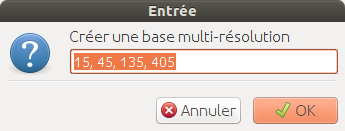
\includegraphics[scale=0.5]{img/gen_ms-fr.png} 
	\caption{Génération d'une base multi-résolution}
\end{figure}

Il est conseillé d'utiliser des résolutions qui suivent une suite géométrique d'un facteur 2, 3 ou 4.
PixScape va créer un nouveau MNT pour chaque résolution, ainsi que le MNE et l'occupation du sol si ces couches sont présentes dans le projet.
Pour le MNT et le MNE les pixels sont agrégés par la moyenne arithmétique, pour l'occupation du sol, les pixels sont agrégés par le mode \textit{ie.} la catégorie d'occupation du sol dominante.
A la fin du traitement, l'ensemble des nouvelles couches sont enregistrées au format Tiff dans le répertoire du projet et sont ajoutés dans l'arborescence des couches de la fenêtre principale.


\subsubsection{Importer les données}
La base multi-résolution peut être importée pour chaque résolution. Il faudra fournir au minimum le MNT plus le MNE et l'occupation du sol si ces couches sont déjà présentes pour la résolution initiale. Comme à la création du projet, la résolution des altitudes du MNT peut être renseignée. 

\begin{figure}[H]
	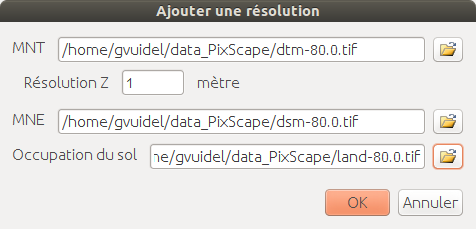
\includegraphics[scale=0.5]{img/add_scale-fr.png} 
	\caption{Import des couches pour une résolution}
\end{figure}

La résolution des hauteurs du MNE doit être obligatoirement en mètre et les codes d'occupation du sol doivent être compris entre 0 et 255. Pour l'occupation du sol, les codes peuvent varier d'une résolution à une autre pour différencier des objets qui n'ont pas la même signification selon la résolution, par exemple un arbre et une forêt, un bâtiment et un village.  
Les 3 couches doivent avoir exactement la même géométrie : la même emprise spatiale et la même résolution.
Enfin, l'emprise spatiale doit couvrir au minimum l'emprise spatiale des données initiales. 

A partir du moment où le projet contient des données multi-résolution, elles pourront être utilisées dans les calculs de visibilité en activant le paramètre Multi-résolution dans la fenêtre Options (voir \nameref{options}). 

\section{Calcul de visibilité}

Deux méthodes de calcul de visibilité sont accessibles à partir du menu Visibilité : la vue planimétrique et la vue tangentielle.
Pour chacune des deux méthodes, l'utilisateur peut visualiser le résultat de manière interactive pour un point d'observation donné en cliquant sur la carte.

\subsection{Vue planimétrique}
La vue planimétrique correspond à la surface sur le plan (x,y) contenant l'ensemble des points visibles à partir du point d'observation O. Le résultat est appelé bassin de visibilité ou viewshed en anglais (cf. figure \ref{viewshed}).

\begin{figure}[H]
	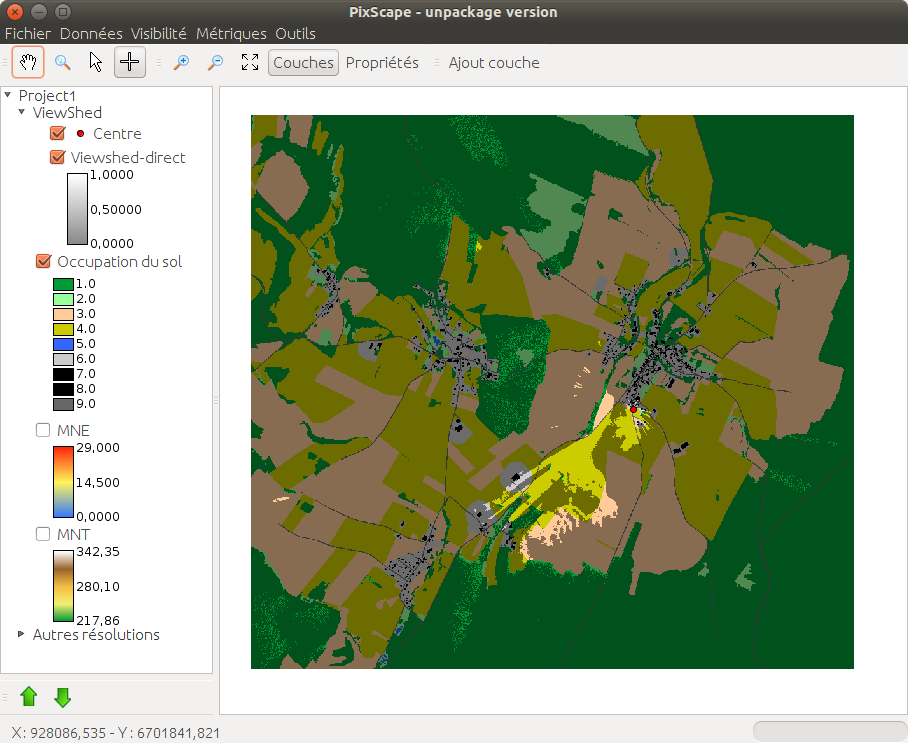
\includegraphics[scale=0.5]{img/viewshed-fr.png} 
	\caption{Résultat d'une vue planimétrique à partir du point rouge. Le bassin de visibilité est affiché par transparence.}
	\label{viewshed}
\end{figure}

Le calcul d'une vue planimétrique est accessible à partir du menu Visibilité / Vue planimétrique. Une fenêtre apparaît montrant l'ensemble des paramètres rentrant en ligne de compte pour le calcul d'un bassin de visibilité (figure \ref{viewshed_param_fig}). 

\begin{figure}[H]
	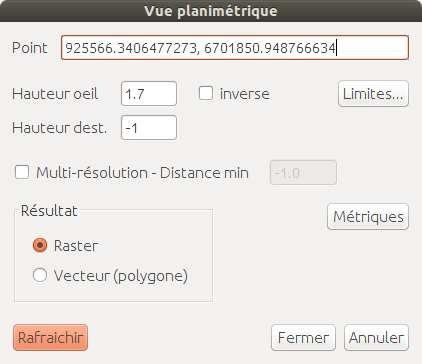
\includegraphics[scale=0.5]{img/viewshed_dlg-fr.png} 
	\caption{Paramétrage de la vue planimétrique}
	\label{viewshed_param_fig}
\end{figure}

\subsubsection{Paramètres}
\label{viewshed_param}
\begin{itemize}
	\item Point : coordonnées du point d'observation ou observé O. Il peut être saisi manuellement ou bien donné directement en cliquant sur la carte.
	\item Hauteur oeil (h1) : hauteur en mètre de l'oeil de l'observateur
	\item Hauteur dest. (h2) : hauteur en mètre du ou des points observés. S'il est défini à -1, la hauteur du MNE est utilisée. Dans le cas où le projet ne contient pas de MNE, la hauteur est nulle.
	\item Inverse : par défaut la case est décochée, le point O est le point d'observation \textit{ie.} l'oeil de l'observateur (figure \ref{height_view}). Le bassin de visibilité correspond à l'ensemble des points visible depuis O. A l'inverse, si la case est cochée, le point O devient le point observé (figure \ref{height_view_inverse}). Le bassin de visibilité correspond alors à l'ensemble des points d'où l'observateur voit le point O.
	\item Limites : cette fenêtre permet de restreindre le champ de vision de l'observateur dans les 3 dimensions (voir \nameref{bounds})
	\item Multi-résolution : active ou désactive le calcul en multi-résolution. S'il est activé, la distance minimale en mètre avant le changement de résolution doit être indiquée.
\end{itemize}


\begin{figure}[H]
	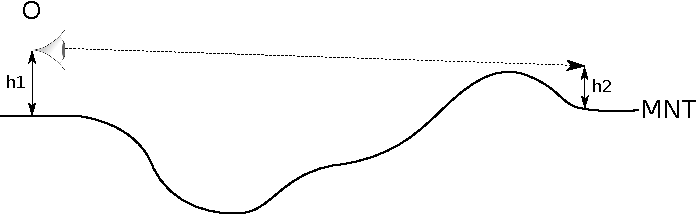
\includegraphics{img/height_view.pdf} 
	\caption{Mode par défaut : O est le point d'observation, h1 est la hauteur de l'oeil et h2 la hauteur à la destination ou la hauteur du MNE si Hauteur dest. = -1}
	\label{height_view}
\end{figure}

Le paramètre Hauteur dest. (h2) est souvent utilisé en conjonction du mode inverse pour analyser l'impact d'une construction (pylone, éolienne, etc). Le bassin de visibilité résultant correspond alors aux points à partir desquels la nouvelle construction d'une hauteur h2 sera visible (figure \ref{height_view_inverse}).

\begin{figure}[H]
	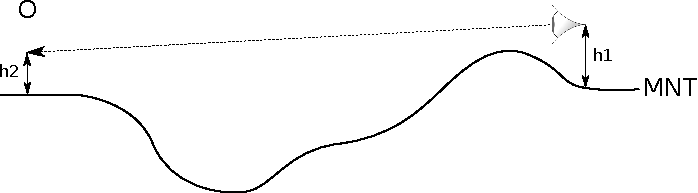
\includegraphics{img/height_view_inverse.pdf} 
	\caption{Mode inverse : O est le point observé, h1 est la hauteur de l'oeil et h2 la hauteur à la destination (défini par Hauteur dest. ou la hauteur du MNE si Hauteur dest. = -1)}
	\label{height_view_inverse}	
\end{figure}

\subsubsection{Résultats}

Le bassin de visibilité peut être affiché sur la carte en raster ou en vectoriel selon le choix effectué dans le panneau Résultat. En raster, les zones de couleurs vives correspondent au zones visibles. A l'inverse, en vectoriel, les zones sombres correspondent aux zones visibles. Dans les deux cas, la couche de résultat peut être exportée par un clic droit sur la couche.

Des métriques peuvent être sélectionnées à partir du bouton Métriques pour être calculées sur le bassin de visibilité actuel. Pour plus de détails sur les métriques, voir la section \nameref{metrics}

\begin{figure}[H]
	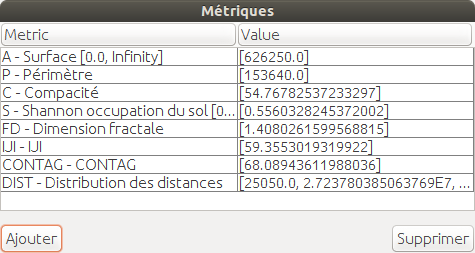
\includegraphics[scale=0.5]{img/viewshed_metric-fr.png} 
	\caption{Métriques calculées à partir du bassin de visibilité}
	\label{viewshed_metric}
\end{figure}

Après avoir modifié un paramètre, il suffit de cliquer sur le bouton Rafraichir pour que le bassin de visibilité soit mis à jour sur la carte ainsi que les métriques si elles sont affichées.

\subsection{Vue tangentielle}

Le calcul d'une vue tangentielle est accessible à partir du menu Visibilité / Vue tangentielle. Une fenêtre apparaît montrant les paramètres pour le calcul de la vue ainsi que pour l'affichage du résultat (figure \ref{viewtan_param}). 

\begin{figure}[H]
	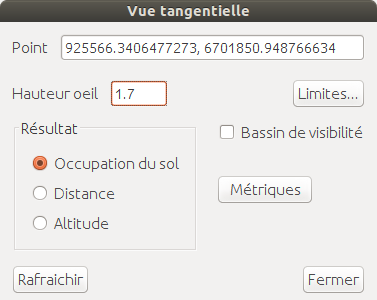
\includegraphics[scale=0.5]{img/viewtan_dlg-fr.png} 
	\caption{Paramétrage de la vue tangentielle}
	\label{viewtan_param}
\end{figure}

\subsubsection{Paramètres}

\begin{itemize}
	\item Point : coordonnées du point d'observation O. Il peut être saisi manuellement ou bien donné directement en cliquant sur la carte.
	\item Hauteur oeil (h1) : hauteur en mètre de l'oeil de l'observateur
	\item Limites : cette fenêtre permet de restreindre le champ de vision de l'observateur dans les 3 dimensions (voir \nameref{bounds})
	\item Bassin de visibilité : si ce paramètre est coché, le bassin de visibilité est affiché sur la carte.
	\item Résultat : choix de l'affichage du résultat (voir \nameref{viewtan_result}).
\end{itemize}

Le paramétrage de la résolution angulaire ainsi que l'utilisation d'une base multi-résolution n'est pas accessible dans cette fenêtre mais uniquement dans la fenêtre des Options (voir \nameref{options}).

\subsubsection{Résultats}
\label{viewtan_result}
Le résultat est affiché dans une nouvelle fenêtre représentant la vue tangentielle (figure \ref{viewtan_land}). Les coordonnées de cette image sont en degré de -180° à +180° à l'horizontal et de -90° à +90° à la verticale, le nord étant à 0° au milieu de l'image. 

\begin{figure}[H]
	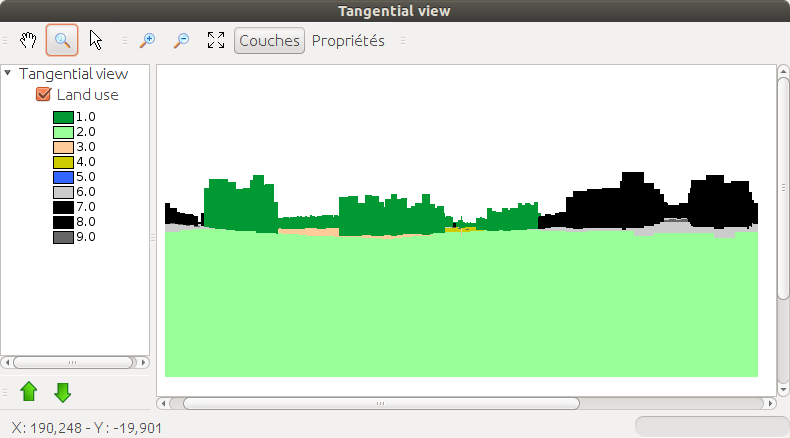
\includegraphics[scale=0.5]{img/viewtan_land-fr.png} 
	\caption{Résultat d'une vue tangentielle. Les couleurs représentent l'occupation du sol.}
	\label{viewtan_land}
\end{figure}

Par défaut, les couleurs représentent les catégories d'occupation du sol (figure \ref{viewtan_land}). En sélectionnant Distance dans le panneau résultat, la vue tangentielle affiche les distances au point d'observation (figure \ref{viewtan_dist}).

\begin{figure}[H]
	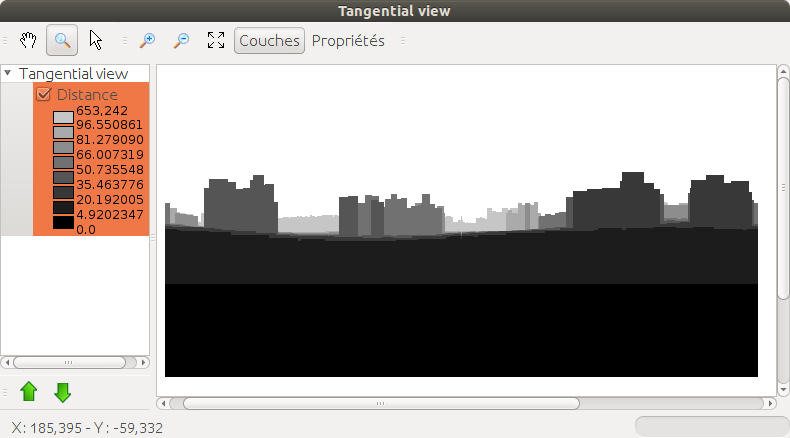
\includegraphics[scale=0.5]{img/viewtan_dist-fr.png} 
	\caption{Résultat d'une vue tangentielle. Les couleurs représentent la distance au point d'observation.}
	\label{viewtan_dist}
\end{figure}

Des métriques peuvent être sélectionnées à partir du bouton Métriques pour être calculées sur la vue tangentielle actuelle. Pour plus de détails sur les métriques, voir la section \nameref{metrics}

Après avoir modifié un paramètre, il suffit de cliquer sur le bouton Rafraichir pour que la vue soit mis à jour sur la carte ainsi que les métriques si elles sont affichées.

\subsection{Bassins multiples}
\label{multi_viewshed}
Le menu Visibilité / Bassins multiples permet de calculer plusieurs bassins de visibilité en une fois à partir d'un shapefile contenant les points d'observation.

\begin{figure}[H]
	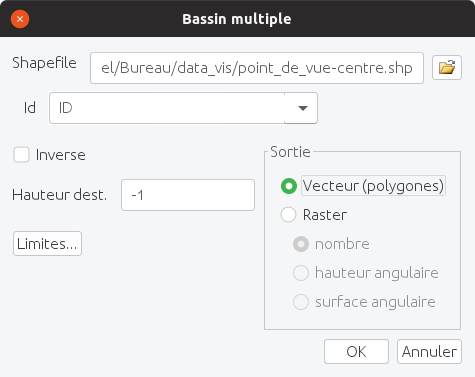
\includegraphics[scale=0.5]{img/multi_viewshed-fr.png} 
	\caption{Fenêtre de paramétrage des bassins multiples}
	\label{multi_viewshed_dlg}
\end{figure}

\subsubsection{Paramètres}

\begin{itemize}
	\item Shapefile : shapefile contenant les points d'observation.
	\item id : attribut du shapefile identifiant chaque point. Ce paramètre est utile uniquement pour un résultat en vectoriel.
	\item Inverse : par défaut la case est décochée, les points représentent les points d'observation \textit{ie.} l'oeil de l'observateur. A l'inverse, si la case est cochée, les points correspondent aux points observés. Pour plus de détails voir \nameref{viewshed_param} de la vue planimétrique.
	\item Hauteur dest. (h2) : hauteur en mètre du ou des points observés. Si il est défini à -1, la hauteur du MNE est utilisée. Dans le cas où le projet ne contient pas de MNE la hauteur est nulle.
	\item Limites : cette fenêtre permet de restreindre le champ de vision de l'observateur dans les 3 dimensions pour tous les points d'observation (voir \nameref{bounds}). Si le shapefile contient les attributs (dmin, dmax, zmin, zmax, orien et amp), ils seront utilisés à la place.
	\item Sortie : choix du format de la couche résultat : vecteur ou raster.
	\item Raster : en raster, le résultat peut être le nombre de points visibles (nombre) ou bien la surface angulaire totale visible (surface en degré carré).
\end{itemize}

Le paramétrage de la hauteur de l'observateur ainsi que l'utilisation d'une base multi-résolution n'est pas accessible dans cette fenêtre mais uniquement dans la fenêtre des Options (voir \nameref{options}).

\subsubsection{Résultat}
Les bassins de visibilité peuvent être affichés sur la carte en raster ou en vectoriel selon le choix effectué dans le panneau Sortie. Dans les deux cas, la couche de résultat peut être exportée par un clic droit sur la couche.

En vectoriel, la couche contient un polygone multiple pour chaque bassin de visibilité (figure \ref{multi_viewshed_vector}). Chaque multi-polygone a un attribut Id permettant de faire le lien avec l'identifiant du point d'observation correspondant.

\begin{figure}[H]
	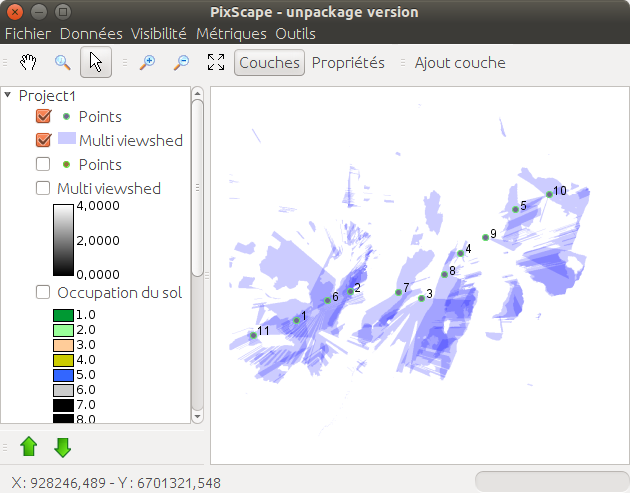
\includegraphics[scale=0.5]{img/multi_viewshed_vector-fr.png} 
	\caption{Résultat vectoriel du calcul de bassins multiples}
	\label{multi_viewshed_vector}
\end{figure}

En raster, la valeur du pixel correspond au nombre de fois où le pixel est contenu dans un bassin de visibilité \textit{ie.} le nombre de points d'observation voyant le pixel ou bien, en mode inverse, le nombre de points d'observation vus par le pixel (figure \ref{multi_viewshed_raster}). Si l'option "surface en degré carré" est sélectionnée, la valeur du pixel n'est plus un nombre de points visibles mais la surface angulaire totale visible en degré carré (figure \ref{multi_viewshed_raster_deg}).

\begin{figure}[H]
	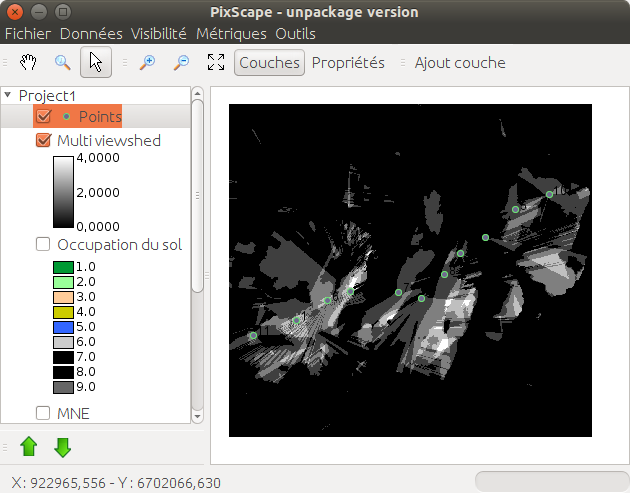
\includegraphics[scale=0.5]{img/multi_viewshed_raster-fr.png} 
	\caption{Résultat raster du calcul de bassins multiples - Hauteur dest. (h2) = -1 - nombre de points}
	\label{multi_viewshed_raster}
\end{figure}

\begin{figure}[H]
	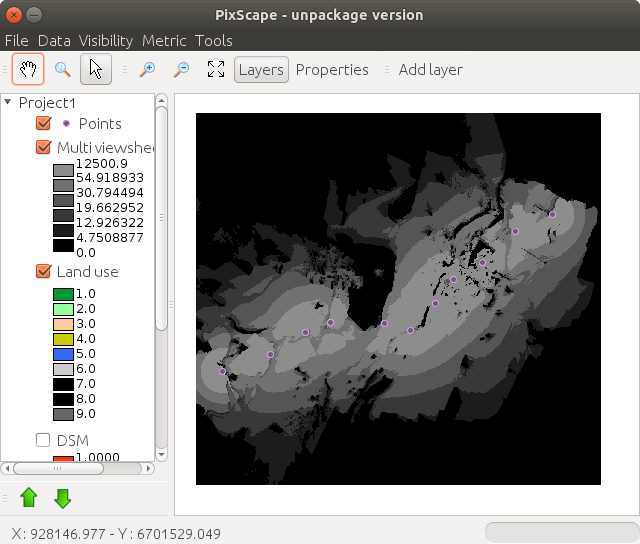
\includegraphics[scale=0.5]{img/multi_viewshed_raster_deg-fr.png} 
	\caption{Résultat raster du calcul de bassins multiples - Hauteur dest. (h2) = 200 - surface en degré}
	\label{multi_viewshed_raster_deg}
\end{figure}

\subsection{Limitation du champ de vision}
\label{bounds_ui}
Pour tous les calculs de visibilité intégrés dans PixScape, le champ de vision peut être restreint dans les 3 dimensions. Le détail est décrit dans la section \nameref{bounds}.

Ces limites peuvent être données à partir de la fenêtre Limites (figure \ref{bounds_dlg}). Dans le cas où les points d'observation sont donnés à partir d'un shapefile, le paramétrage du champ de vision peut être différencié pour chaque point en ajoutant les 6 paramètres (dmin, dmax, zmin, zmax, orien, amp) dans la table des attributs du shapefile. Le menu "Ajouter les attributs" permet de les ajouter automatiquement dans un shapefile existant (voir \nameref{add_attributes}).

\begin{figure}[H]
	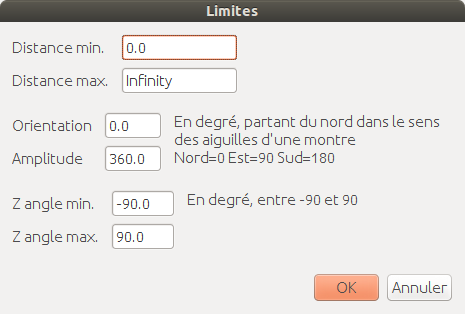
\includegraphics[scale=0.5]{img/bounds-fr.png} 
	\caption{Paramétrage des limites du champ de vision. Par défaut le champ de vision est complet.}
	\label{bounds_dlg}
\end{figure}

\section{Calcul de métriques de visibilité}
\label{calc_metrics}
Dans PixScape, il est possible de synthétiser le résultat d'une vue planimétrique ou tangentielle par un certain nombre d'indicateurs ou métriques. Les métriques disponibles sont détaillées dans le chapitre \nameref{metrics}. 

Le menu Visibilité permet déjà de calculer plusieurs métriques sur la vue courante. Mais ce fonctionnement "manuel" est envisageable pour seulement quelques points d'observation. 

Le menu Métriques, quant à lui, permet de lancer un calcul de visibilité (planimétrique ou tangentielle) ainsi que le calcul des métriques, pour un ensemble de points d'observation en une seule exécution. 

\begin{figure}[H]
	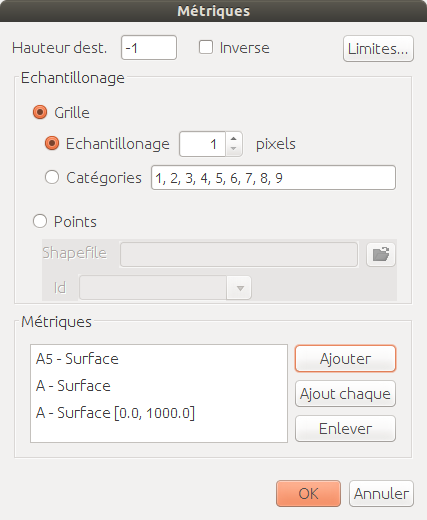
\includegraphics[scale=0.5]{img/metrics-fr.png} 
	\caption{Paramétrage du calcul de métriques}
	\label{metrics_dlg}
\end{figure}

\subsection{Paramétrage de la vue}
Les paramètres spécifiques à la vue sont affichés en haut de la fenêtre (figure \ref{metrics_dlg}) et dépendent du type de vue sélectionné dans le menu Métriques : planimétrique ou tangentiel.

\begin{itemize}
	\item Inverse (planimétrique uniquement) : par défaut la case est décochée, les points représentent les points d'observation \textit{ie.} l'oeil de l'observateur. A l'inverse, si la case est cochée, les points correspondent aux points observés. Pour plus de détails voir \nameref{viewshed_param} de la vue planimétrique.
	\item Hauteur dest. (h2) (planimétrique uniquement) : hauteur en mètre du ou des points observés. S'il est défini à -1, la hauteur du MNE est utilisée. Dans le cas où le projet ne contient pas de MNE la hauteur est nulle.
	\item Limites : cette fenêtre permet de restreindre le champ de vision de l'observateur dans les 3 dimensions pour tous les points d'observation (voir \nameref{bounds}). Si les points sont définis par un shapefile et qu'il contient les attributs (dmin, dmax, zmin, zmax, orien et amp), ils seront utilisés à la place.
\end{itemize}
Les autres paramètres pour la vue (\textit{eg.} hauteur de l'oeil) doivent être définis en amont dans la fenêtre Options (cf. \nameref{options}).

\subsection{Echantillonnage}
\label{sampling}
Les points d'observation peuvent être donnés en raster (option Grille) ou en vectoriel (option Points). Le format du résultat (raster ou vectoriel) est lié au type choisi.

\subsubsection{Échantillonnage raster}
En raster, l'échantillonnage des points d'observation se fait à partir de la grille du MNT à la résolution la plus fine. Deux options sont possibles : un échantillonnage régulier sur la grille ou bien par catégorie d'occupation du sol.

Par défaut, l'échantillonnage est régulier et fixé à 1 pixel, ce qui correspond à un parcours exhaustif de l'ensemble des pixels de l'image \textit{ie.} un calcul de visibilité sera exécuté à partir de chaque pixel comme point d'observation. Si on augmente l'échantillonnage à 3, un pixel sur 3 seulement sera utilisé dans chaque dimension, donc on calculera une vue uniquement pour 1 pixel sur 9 de la grille (figure \ref{grid_sampling}).

\begin{figure}[H]
	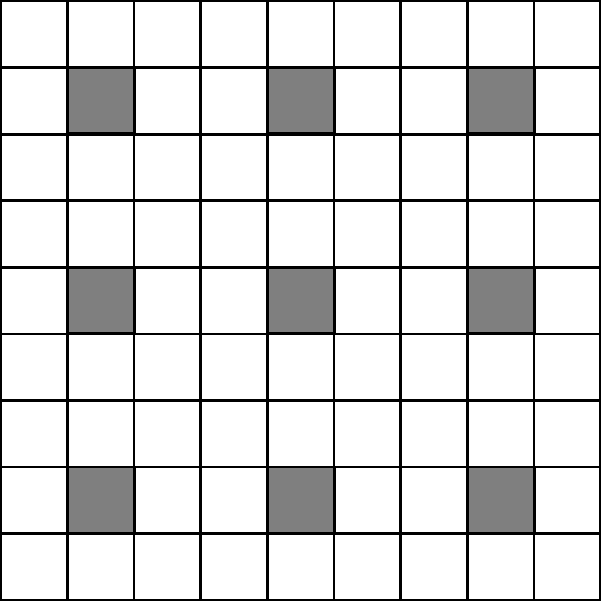
\includegraphics[scale=0.5]{img/grid_sampling.pdf} 
	\caption{Echantillonnage tous les 3 pixels. 9 vues seront calculées à partir des 9 pixels grisés.}
	\label{grid_sampling}
\end{figure}

Si l'échantillonnage se fait par catégorie d'occupation du sol, les vues seront calculées uniquement à partir des pixels appartenant aux catégories listées. Les codes d'occupation du sol doivent être séparés par des virgules.

Le résultat sera sous forme de plusieurs couches raster. Il contiendra une couche pour chaque métrique et pour chaque intervalle de distance défini dans le paramétrage des métriques.

\subsubsection{Échantillonnage vectoriel}
Au lieu d'utiliser la grille raster, on peut fournir un ensemble de points à partir d'un shapefile.

Le résultat sera sous la forme d'une couche de points correspondant au shapefile donné en entrée. Le résultat des métriques sera stocké dans la table attributaire de la couche.


\subsection{Paramétrage des métriques}
\label{param_metrics}
Pour chaque point d'observation, un ensemble de métriques pourra être calculé. Le panneau Métriques permet de les sélectionner et de paramétrer les distances et les catégories d'occupation du sol selon le cas. Une même métrique peut être ajoutée plusieurs fois avec un paramétrage différent.

\begin{figure}[H]
	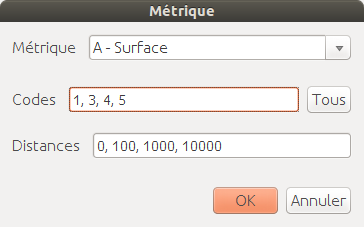
\includegraphics[scale=0.5]{img/metric_param-fr.png} 
	\caption{Paramétrage de la métrique A}
	\label{metric_param_dlg}
\end{figure}

La figure \ref{metric_param_dlg} montre le paramétrage de la métrique A. Dans cet exemple, la métrique A sera calculée uniquement sur les classes d'occupation du sol 1, 3, 4 et 5 pour 3 intervalles de distance [0-100[, [100-1000[ et [1000-10000[. Le résultat contiendra pour chaque point d'observation 3 valeurs, une pour chaque intervalle de distance.

Le bouton "Ajout chaque" permet d'ajouter une métrique plusieurs fois : pour chaque catégorie d'occupation du sol sélectionnée.

Les catégories d'occupation du sol peuvent aussi être regroupées pour ne former qu'une seule classe dans le calcul d'une métrique avec le caractère "-" (figure \ref{metric_param_group_dlg}). Cela permet de garder une occupation du sol détaillée et dans le même temps réaliser certaines analyses sur des classes plus générales.

\begin{figure}[H]
	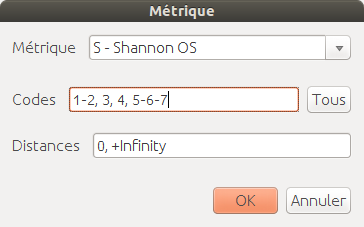
\includegraphics[scale=0.5]{img/metric_param_group-fr.png} 
	\caption{Paramétrage de la métrique S. Les catégories d'occupation du sol sont regroupées en 4 classes.}
	\label{metric_param_group_dlg}
\end{figure}

Le regroupement des catégories d'occupation du sol n'est pas utile pour la métrique A. En effet cette métrique ne différencie pas les catégories sélectionnées en classe. Par exemple, \verb|1,3,4,5| et \verb|1-3,4-5| donnera le même résultat.

\subsection{Résultats}

Le résultat du calcul de métriques est affiché sur la carte par une ou plusieurs couches au format raster ou vectoriel selon le format d'entrée utilisé pour l'échantillonnage. Chaque couche est exportable par un clic droit sur le nom de la couche et le menu "Exporter...".

\subsubsection{Raster}
En raster, le résultat correspond à un ensemble de couche raster, une pour chaque métrique et chaque intervalle de distance. Chaque couche peut être exportée au format Tiff ou AsciiGrid.

A partir du paramétrage de la figure \ref{metric_param_dlg}, PixScape produit 3 couches raster (figure \ref{metric_result_rast}) pour les 3 intervalles de distances donnés.

Si l'échantillonnage sur la grille est supérieur à 1, la taille des pixels sera augmentée proportionnellement au facteur d'échantillonnage.

\begin{figure}[H]
	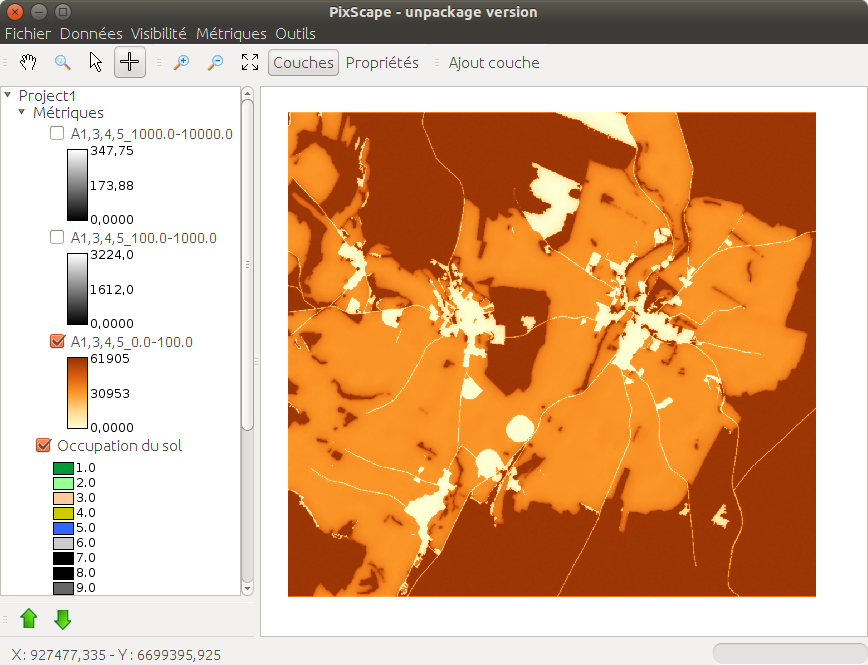
\includegraphics[scale=0.5]{img/metric_result_rast-fr.png} 
	\caption{Résultat d'un calcul de métriques par un échantillonnage sur la grille.}
	\label{metric_result_rast}
\end{figure}

\subsubsection{Vectoriel}

En vectoriel, le résultat est une couche de point contenant les valeurs des métriques dans la table attributaire (figure \ref{metric_result_attr}). Par défaut la première métrique est affichée par cercle proportionnel (figure \ref{metric_result_vect}). Pour afficher une autre métrique, il suffit de modifier l'attribut sélectionné dans l'onglet "Cercle" de la fenêtre de paramétrage du style de la couche.

\begin{figure}[H]
	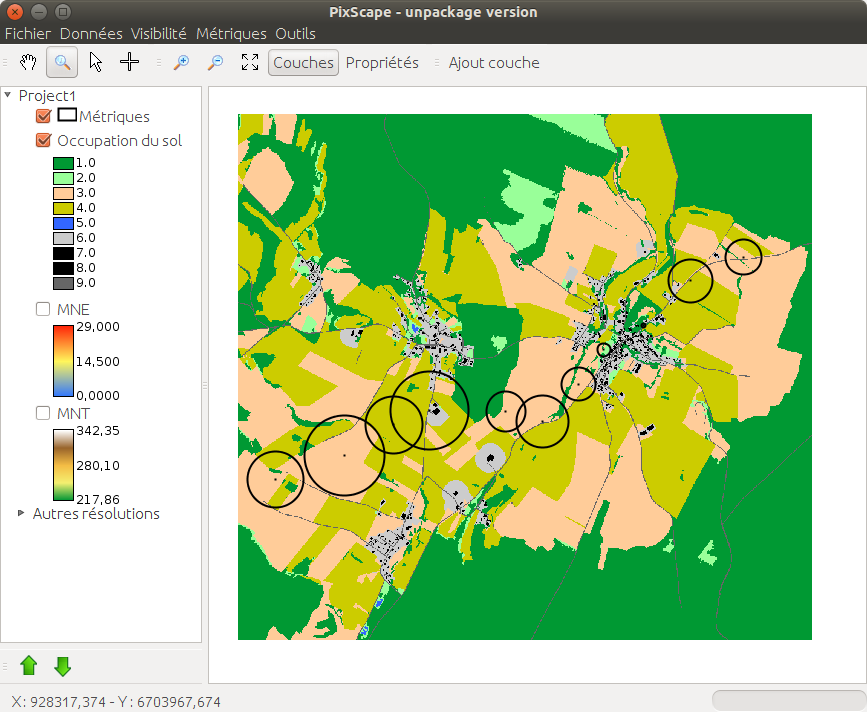
\includegraphics[scale=0.5]{img/metric_result_vect-fr.png} 
	\caption{Résultat d'un calcul de métriques à partir d'un shapefile de point. La première métrique est affichée par des cercles proportionnels à la valeur de la métrique.}
	\label{metric_result_vect}
\end{figure}

La couche "Métriques" peut être exportée au format shapefile ou bien texte par un clic droit sur le nom de la couche et le menu "Exporter...".

\begin{figure}[H]
	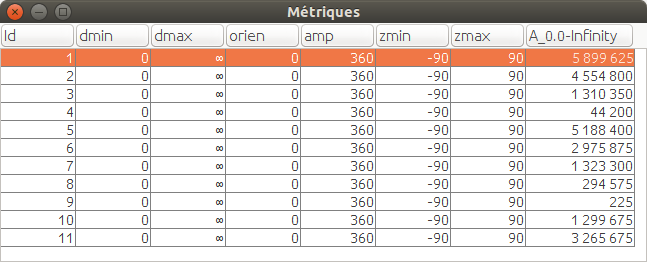
\includegraphics[scale=0.5]{img/metric_result_attr-fr.png} 
	\caption{Table attributaire de la couche résultat}
	\label{metric_result_attr}
\end{figure}

La table attributaire de la couche résultat est accessible par un clic droit sur le nom de la couche et le menu "Table attributaire". Elle contient toujours, en plus des métriques, les 6 paramètres de limitation du champ de vision, permettant de conserver l'information de paramétrage avec les résultats.

\section{Outils et options}
\label{tools}

\subsection{Ajout des attributs du champ de vision}
\label{add_attributes}
Pour l'ensemble des calculs de visibilité, le champ de vision peut être restreint par la fenêtre Limites (figure \ref{bounds_dlg}). Cette solution est pratique quand pour chaque point d'observation les même restrictions du champ de vision s'appliquent. 
Le menu Outils / Ajouter les attributs est utile quant à lui pour spécifier des restrictions différentes pour chaque point d'observation. Cette fonction ajoute les 6 attributs à un shapefile avec les valeurs par défaut définies par la fenêtre Limites. Vous pouvez ensuite avec votre SIG préféré modifier les valeurs de restriction pour chaque point d'observation. 
Le shapefile en sortie pourra être utilisé pour le calcul de métriques (\ref{calc_metrics}) et le calcul de bassins multiples (\ref{multi_viewshed}) qui tiendront compte des restrictions du champ de vision différenciées pour chaque point.

\begin{figure}[H]
	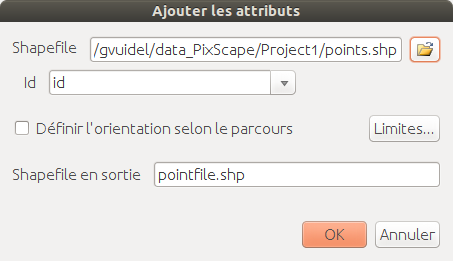
\includegraphics[scale=0.5]{img/add_attributes-fr.png} 
	\caption{Ajout des attributs à un shapefile pour limiter le champ de vision}
	\label{add_attributes_dlg}
\end{figure}

\subsubsection{Champ de vision le long d'un parcours}
La case à cocher "Définir l'orientation selon le parcours" calcule l'orientation de chaque point par rapport au suivant. Avec cette option, le paramètre orientation de la fenêtre Limites sera ignoré et chaque point aura potentiellement une valeur d'orientation différente. 

\begin{figure}[H]
	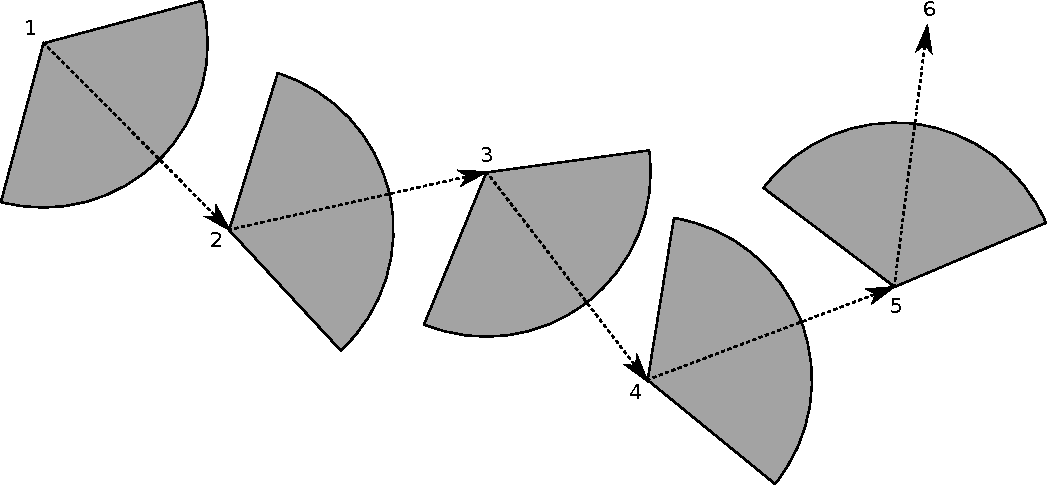
\includegraphics[scale=0.8]{img/path_orien.pdf} 
	\caption{Champ de vision le long d'un parcours. L'orientation est calculée en direction du point suivant et l'amplitude est constante.}
	\label{path_orien}
\end{figure}

L'ordre des points est défini par l'attribut id qui est trié par ordre croissant.
Cette option est utile uniquement avec une amplitude inférieure à 360°.


\subsection{Options}
\label{options}
Les options générales du projet sont accessibles à partir du menu Outils / Options.
Ces options sont enregistrées automatiquement dans le fichier xml du projet. Elles sont utilisées pour l'ensemble des calculs de visibilité sauf quand l'option est aussi présente dans la fenêtre de paramétrage d'un traitement. Par exemple, la hauteur de l'oeil est modifiable directement dans la fenêtre de paramétrage d'une vue planimétrique ou tangentielle, mais elle ne l'est pas pour le calcul des métriques. Dans ce dernier cas, la hauteur de l'oeil de l'observateur sera celle définie dans la fenêtre d'options.

\begin{figure}[H]
	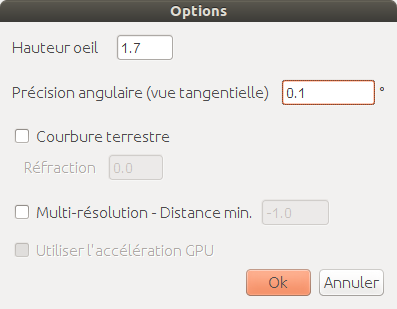
\includegraphics[scale=0.5]{img/options-fr.png} 
	\caption{Options générales}
\end{figure}

\subsubsection{Hauteur de l'oeil de l'observateur}
Le paramètre Hauteur oeil ($h1$) spécifie la hauteur de l'observateur à partir du MNT. L'unité est le mètre. Pour plus de détails, voir \nameref{principles} et la figure \ref{ray_side}.

\subsubsection{Précision angulaire}
Le paramètre Précision angulaire ($\alpha$) définit la résolution en degré de la vue tangentielle. Il est fixé par défaut à 0.1°, ce qui correspond à 3600 rayons calculés si l'amplitude de la vue est à 360°. Pour plus de détails, voir \nameref{principles_tan} et la figure \ref{grid_tan}. 

\subsubsection{Courbure terrestre}
\label{curvature}
Les calculs de visibilité dans PixScape peuvent tenir compte de la courbure de la Terre, susceptible de jouer un rôle dans le cas d'une vue à plusieurs dizaines de kilomètres. Le principe du calcul est simple : plus la distance à l'observateur augmente, plus la hauteur des objets visibles diminuent. 
La hauteur tenant compte de la courbure de la Terre $z'_i$ d'un point $i$ est calculée comme suit : 

$$z'_i = z_i - \frac{d_i^2}{D}$$

avec $z_i$ l'altitude du MNT au point $i$, $d_i$ la distance entre le point $i$ et l'observateur et $D$ le diamètre de la Terre (12 740 000 mètres).

La courbure de la Terre peut être compensée en partie par la réfraction de la lumière dans l'atmosphère. Dans PixScape, à partir du moment où la courbure terrestre est prise en compte, le paramètre de réfraction peut être spécifié. Il est défini par défaut à 0,13. Le calcul de la hauteur devient : 

$$z'_i = z_i - (1-\rho)\frac{d_i^2}{D}$$

avec $\rho$ le coefficient de réfraction compris entre 0 et 1. Si $\rho=0$ on retombe sur la formule précédente sans réfraction.


\subsubsection{Multi-résolution}
A partir du moment où le projet contient les données à plusieurs résolutions, les calculs de visibilité peuvent se faire en multi-résolution en activant cette option. Le paramètre de distance minimale est à définir obligatoirement. Il permet d'assurer une distance minimale en mètre avant de changer de résolution. 

Pour plus de détails sur le calcul de visibilité en multi-résolution, voir \nameref{multires}.


\subsubsection{Accélération GPU}
Ce paramètre permet de réaliser les calculs de visibilité sur la carte graphique au lieu du processeur. Les gains en temps d'exécution peuvent être importants pour des cartes graphiques Nvidia de la gamme Tesla, conçues pour le calcul haute performance (voir \nameref{perf}). En revanche, toutes les métriques ne sont pas optimisées pour le GPU. Les métriques A et S sont les seules à être optimisées. Si vous utilisez d'autres métriques, les gains de temps seront minimes voire inexistants.

Le paramètre est grisé si PixScape ne peux pas utiliser l'accélération GPU. Les causes peuvent être multiples : pas de carte graphique NVidia, pas de support de CUDA, pas la bonne version de CUDA (6.5).

Si l'option multi-résolution est active, l'accélération GPU ne sera pas utilisée même si elle est activée.


\chapter{Interface en ligne de commande}
\label{cli}

Dès lors qu'un projet a été créé depuis l'interface graphique, il est possible d'utiliser PixScape en ligne de commande. Ce mode est utile pour exécuter le logiciel sur un ordinateur distant sans interface graphique, lancer automatiquement plusieurs traitements à la suite, ou encore soumettre des exécutions sur un cluster.

\section{Démarrage}

\subsection{Lancer PixScape en ligne de commande}
Il faut tout d'abord ouvrir une fenêtre de terminal, puis aller dans le répertoire contenant PixScape avec la commande \textit{cd}.
Enfin, vous pouvez saisir la commande suivante pour afficher l'écran d'aide de PixScape :
\begin{Verbatim}
java -jar pixscape.jar --help
\end{Verbatim}
Résultat
\begin{Verbatim}
Usage :
java -jar pixscape.jar --metrics
...
...
\end{Verbatim}
Vous êtes prêt à utiliser PixScape en ligne de commande.

\subsection{Syntaxe}
\subsubsection{Définition}
Les commandes commencent par un double tiret : \verb|--project, --metrics, ...|\\
Les options globales commencent par un tiret simple : \verb|-proc, -bounds, ...|\\
Les paramètres n'ont pas de tiret : \verb|dmin, inverse, ...|

\subsubsection{Séparateur}
Les espaces sont utilisés pour séparer les différents éléments d'une ligne de commande, par conséquent, vous ne pouvez pas avoir un nom qui contient des espaces.\\

\subsubsection{Syntaxe de l'écran d'aide}
Dans l'écran d'aide, les éléments entourés de crochets sont optionnels, et donc les éléments qui ne sont pas entourés par des crochets sont obligatoires. Le caractère \verb+|+ sépare les options possibles.

\section{Commandes}

\subsection{--help : affichage de l'aide}
Commande :
\begin{Verbatim}
java -jar pixscape-1.1.jar --help
\end{Verbatim}
Résultat :
\begin{Verbatim}
Usage :
java -jar pixscape.jar --metrics
java -jar pixscape.jar [-mpi | -proc n | -cuda n]
--project project_file.xml
[--landmod zone=filezones.shp id=fieldname code=fieldname dsm=file.tif [selid=id1,...,idn]]
[-zeye val] [-zdest val] [-resdir path]
[-bounds [dmin=val] [dmax=val] [orien=val] [amp=val] [zmin=val] [zmax=val]]
[-sampling n=val | land=code1,..,coden | points=pointfile.shp id=fieldname]
[-multi dmin=val | -mono]
[-earth flat|curved [refrac=val]]
commands

Commands list :
--viewshed [inverse] x y [resfile=raster.tif]
--viewtan [prec=deg] x y [resname=name]
--multiviewshed format=vector|raster [inverse] [degree] [resname=name]
--planmetric [inverse] metric1[[code1,...,coden]][_d1,...,dm] ... metricn[[code1,...,coden]][_d1,...,dm]
--tanmetric [prec=deg] metric1[[code1,...,coden]][_d1,...,dm] ... metricn[[code1,...,coden]][_d1,...,dm]
--toobject [degree] [agreg=eye|object] objects=pointfile.shp id=fieldname [resname=name]
\end{Verbatim}

\subsection{--metrics : affichage des métriques}
Cette commande affiche l'ensemble des métriques disponibles avec leur abréviation et leur nom. 

Commande :
\begin{Verbatim}
java -jar pixscape-1.1.jar --metrics
\end{Verbatim}
Résultat :
\begin{Verbatim}
===== Metrics =====
A - Surface
S - Shannon OS
P - Périmètre
C - Compacité
FD - Dimension fractale
AG - Indice d'agrégation
CONTAG - Contagion
ED - Densité de bords
PD - Densité de taches
PMS - Taille moyenne des taches
DIST - Distribution des distances
SL - Ligne d'horizon
SD - Shannon profondeur
DL - Profondeur de vue
\end{Verbatim}

\subsection{--project : chargement d'un projet}
Cette commande définit le chemin vers le fichier xml du projet à charger.
\begin{Verbatim}[commandchars=\\\{\}]
java -jar pixscape-1.1.jar --project \textit{path2myproject/myproject.xml}
\end{Verbatim}
Charge le projet \textit{myproject} contenu dans le répertoire \textit{path2myproject}.

La commande \verb|--project| ne peut être utilisée qu'une seule fois et doit être la première commande de la ligne.
Toutes les commandes qui suivent dans ce manuel ont besoin d'un projet chargé.

\subsection{--landmod : changements d'occupation du sol}

\begin{Verbatim}[commandchars=\\\{\}]
--landmod zone=\textit{filezones.shp} id=\textit{fieldname} code=\textit{fieldname} dsm=\textit{file.tif} [selid=\textit{id1,...,idn}]
\end{Verbatim}

\subsubsection{Paramètres obligatoires}
\begin{itemize}
	\item \verb|zone=filezones.shp| : shapefile de polygones contenant les changements d'occupation du sol
	\item \verb|id=fieldname| : nom d'un attribut du shapefile servant à identifier les polygones. Si les valeurs ne sont pas uniques, les polygones ayant le même identifiant seront appliqués en un seul changement.
	\item \verb|code=fieldname| : nom d'un attribut du shapefile stockant la nouvelle catégorie d'occupation du sol du polygone
	\item \verb|dsm=file.tif| : raster stockant les nouvelles valeurs de MNE utilisées à chaque changement d'occupation du sol. La géométrie du raster doit être exactement la même que le MNT du projet.
\end{itemize}

\subsubsection{Paramètre optionnel}
\begin{itemize}
	\item \verb|selid=id1,...,idn| : liste des identifiants de polygones à traiter. Si ce paramètre n'est pas renseigné tous les polygones du shapefile sont utilisés.
\end{itemize}

\subsubsection{Description}
Cette commande doit être placée avant les commandes de calcul de visibilité. Elle va dupliquer le projet pour chaque polygone du shapefile et modifier l'occupation du sol couvert par le polygone ainsi que le MNE. Les commandes suivant celle-ci seront exécutées sur chaque projet modifié.

Les projets créés seront nommés par l'identifiant du (ou des) polygones et stockés dans le répertoire du projet.

\subsection{--viewshed : vue planimétrique}
\begin{Verbatim}[commandchars=\\\{\}]
--viewshed [inverse] \textit{x} \textit{y} [resfile=\textit{raster.tif}]
\end{Verbatim}

\subsubsection{Paramètres obligatoires}
\begin{itemize}
	\item \verb|x| : abscisse du point d'observation dans le système de coordonnées du MNT
	\item \verb|y| : ordonnée du point d'observation dans le système de coordonnées du MNT
\end{itemize}

\subsubsection{Paramètres optionnels}
\begin{itemize}
	\item \verb|inverse| : passe en mode inverse, le point O devient le point observé
	\item \verb|resfile=raster.tif| : permet de spécifier un autre nom pour le fichier stockant le résultat
\end{itemize}

\subsubsection{Description}
La commande \verb|--viewshed| permet de calculer le bassin de visibilité à partir d'un point d'observation. Le résultat est stocké dans un fichier raster de la même taille que le MNT, au format Tiff. Dans ce raster, le bassin de visibilité est formé des pixels dont la valeur est à 1, les autres sont à 0.

\subsubsection{Exemples}
L'exemple ci-dessous calcule le bassin de visibilité pour un observateur situé au point de coordonnées (925560, 6702495). Le résultat sera stocké dans le répertoire du projet dans un fichier nommé : \verb|viewshed-925560,6702495.tif|.
\begin{Verbatim}
	--viewshed 925560 6702495
\end{Verbatim}

Le second exemple calcule le bassin de visibilité en mode inverse et enregistre le résultat dans le fichier \verb|bassin1.tif|.
\begin{Verbatim}
	--viewshed inverse 925560 6702495 resfile=bassin1.tif
\end{Verbatim}

\subsection{--viewtan : vue tangentielle}
\begin{Verbatim}[commandchars=\\\{\}]
--viewtan [prec=\textit{deg}] \textit{x} \textit{y} [resname=\textit{name}]
\end{Verbatim}

\subsubsection{Paramètres obligatoires}
\begin{itemize}
	\item \verb|x| : abscisse du point d'observation dans le système de coordonnées du MNT
	\item \verb|y| : ordonnée du point d'observation dans le système de coordonnées du MNT
\end{itemize}

\subsubsection{Paramètres optionnels}
\begin{itemize}
	\item \verb|prec=deg| : défini la précision angulaire en degré. Si ce paramètre n'est pas défini, la précision angulaire enregistrée dans le projet sera utilisée.
	\item \verb|resname=name| : permet de spécifier un autre nom pour les fichiers stockant le résultat
\end{itemize}

\subsubsection{Description}
La commande \verb|--viewtan| permet de calculer la vue tangentielle à partir d'un point d'observation. Les résultats sont stockés dans 2 ou 3 fichiers rasters au format Tiff selon si le projet contient une couche d'occupation du sol. 
\begin{itemize}
	\item \verb|elev| : altitude du MNT
	\item \verb|dist| : distance 2D au point d'observation
	\item \verb|land| : occupation du sol, si présent dans le projet
\end{itemize}

La taille des raster dépend de la précision angulaire. Pour une précision de 0,1° et une vue à 360°, les images auront une taille de 3600x1800 pixels. Leur système de coordonnées est défini en degré. 

\subsubsection{Exemples}
L'exemple ci-dessous calcule la vue tangentielle pour un observateur situé au point de coordonnées (925560, 6702495). Le résultat sera stocké dans le répertoire du projet dans les fichiers nommés : \verb|viewtan-925560,6702495-elev.tif|, \verb|viewtan-925560,6702495-dist.tif| et \verb|viewtan-925560,6702495-land.tif| si le projet contient une couche d'occupation du sol.
\begin{Verbatim}
	--viewtan 925560 6702495
\end{Verbatim}

Le second exemple calcule la vue tangentielle avec une précision angulaire de 0,05° et enregistre le résultat dans les fichiers \verb|vue1-elev.tif|, \verb|vue1-dist.tif| et \verb|vue1-land.tif| si le projet contient une couche d'occupation du sol.
\begin{Verbatim}
	--viewtan prec=0.05 925560 6702495 resname=vue1
\end{Verbatim}


\subsection{--multiviewshed : bassin de visibilité multiple}
\begin{Verbatim}[commandchars=\\\{\}]
--multiviewshed format=vector|raster [inverse] [degree] [resname=\textit{name}]
\end{Verbatim}

\subsubsection{Paramètre obligatoire}
\begin{itemize}
	\item \verb/format=vector|raster/ : format du résultat (shapefile ou tiff)
\end{itemize}

\subsubsection{Paramètres optionnels}
\begin{itemize}
	\item \verb|inverse| : passe en mode inverse, le point O devient le point observé
	\item \verb|degree| : pour le format raster, cumule les surfaces visibles en degré carré au lieu du nombre de points visibles. Cette option ne fonctionne qu'en format raster
	\item \verb|resname=name| : permet de spécifier un autre nom pour le fichier stockant le résultat
\end{itemize}

\subsubsection{Description}
La commande \verb|--multiviewshed| permet de calculer les bassins de visibilité à partir d'un ensemble de points d'observation. Les points d'observation doivent être donnés par l'option \verb|-sampling|. Le résultat est stocké dans un fichier raster ou vecteur selon le format choisi. 

En raster, l'image est de la même taille que le MNT, au format Tiff. Dans ce raster, chaque pixel recense le nombre de fois qu'il est vu depuis les points d'observation et en mode inverse le nombre de points vu à partir de ce pixel. Si l'option \verb|degree| est utilisée, chaque pixel représente la surface totale en degré carré de ce pixel visible depuis chaque point d'observation. En mode inverse, chaque pixel contient la surface visible en degré carré depuis ce pixel vers tous les points d'observation.

En vectoriel, le résultat est un shapefile contenant le bassin de visibilité de chaque point d'observation.

\subsubsection{Exemple}
L'exemple ci-dessous calcule les bassins de visibilité des points d'observation donnés dans le shapefile points.shp et stocke le résultat dans un shapefile dans le répertoire du projet nommé : \verb|multiviewshed.shp|.
\begin{Verbatim}
-sampling points=points.shp id=fid --multiviewshed format=vector
\end{Verbatim}


\subsection{--planmetric : métriques en vue planimétrique}

\begin{Verbatim}[commandchars=\\\{\}]
--planmetric [inverse] \textit{metric1}[[\textit{code1,...,coden}]][_\textit{d1,...,dm}] ...
\end{Verbatim}

\subsubsection{Paramètres obligatoires}
\begin{itemize}
	\item \verb|metric1[[code1,...,coden]][_d1,...,dm]| : métrique planimétrique à calculer avec ses paramètres (cf. \nameref{param_metrics_cli}).
	\item ...
\end{itemize}

\subsubsection{Paramètre optionnel}
\begin{itemize}
	\item \verb|inverse| : passe en mode inverse, les points d'observation deviennent les points observés
\end{itemize}

\subsubsection{Description}
La commande \verb|--planmetric| permet de calculer un ensemble de métriques en vue planimétrique. Les points d'observation sont définis en amont par l'option globale \verb|-sampling|. Si l'option n'est pas renseignée, l'échantillonnage par défaut se fait sur la grille pour tous les pixels du MNT ($n=1$).

Les résultats sont stockés dans plusieurs fichiers Tiff pour un échantillonnage sur la grille et dans un shapefile pour un échantillonnage vectoriel.


\subsubsection{Exemples}

L'exemple ci-dessous calcule la métrique A sans paramètre. Si l'échantillonnage est sur la grille, le résultat sera stocké dans le fichier \verb|A-.tif|.
\begin{Verbatim}
	--planmetric A
\end{Verbatim}

L'exemple ci-dessous calcule en vue inversée la métrique A pour le code d'occupation du sol 1 et la métrique A pour le code 2. Si l'échantillonnage est sur la grille, le résultat sera stocké dans les fichiers \verb|A1-.tif| et \verb|A2-.tif|.
\begin{Verbatim}
	--planmetric inverse A[1] A[2]
\end{Verbatim}


\subsection{--tanmetric : métriques en vue tangentielle}
\begin{Verbatim}[commandchars=\\\{\}]
--tanmetric [prec=\textit{deg}] \textit{metric1}[[\textit{code1,...,coden}]][_\textit{d1,...,dm}] ...
\end{Verbatim}

\subsubsection{Paramètres obligatoires}
\begin{itemize}
	\item \verb|metric1[[code1,...,coden]][_d1,...,dm]| : métrique tangentielle à calculer avec ses paramètres (cf. \nameref{param_metrics_cli}).
	\item ...
\end{itemize}

\subsubsection{Paramètre optionnel}
\begin{itemize}
	\item \verb|prec=deg| : précision angulaire en degrés
\end{itemize}

\subsubsection{Description}
La commande \verb|--tanmetric| permet de calculer un ensemble de métriques en vue tangentielle. Les points d'observation sont définis en amont par l'option globale \verb|-sampling|. Si l'option n'est pas renseignée, l'échantillonnage par défaut se fait sur la grille pour tous les pixels du MNT ($n=1$).

Les résultats sont stockés dans plusieurs fichiers Tiff pour un échantillonnage sur la grille et dans un shapefile pour un échantillonnage vectoriel.


\subsubsection{Exemples}

L'exemple ci-dessous calcule la métrique A sans paramètre. Si l'échantillonnage est sur la grille, le résultat sera stocké dans le fichier \verb|A-.tif|.
\begin{Verbatim}
--tanmetric A
\end{Verbatim}

L'exemple ci-dessous calcule les vues tangentielles avec une précision angulaire de 0,05°. La métrique A est calculée 2 fois : pour le code d'occupation du sol 1 et pour le code 2. Si l'échantillonnage est sur la grille, le résultat sera stocké dans les fichiers \verb|A1-.tif| et \verb|A2-.tif|.
\begin{Verbatim}
--tanmetric prec=0.05 A[1] A[2]
\end{Verbatim}


\subsection{--toobject : visibilité point à point}
\begin{Verbatim}[commandchars=\\\{\}]
--toobject [degree] [agreg=eye|object] objects=\textit{pointfile.shp} id=\textit{fieldname} [resname=\textit{name}]
\end{Verbatim}

\subsubsection{Paramètres obligatoires}
\begin{itemize}
	\item \verb|objects=pointfile.shp| : shapefile de points observés
	\item \verb|id=fieldname| : champs du shapefile permettant d'identifier chaque point
\end{itemize}

\subsubsection{Paramètres optionnels}
\begin{itemize}
	\item \verb|degree| : résultat en degré carré
	\item \verb/agreg=eye|object/ : agrégé le résultat par point d'observation (\verb|eye|) ou par point observé (\verb|object|)
	\item \verb|resname=name| : permet de spécifier un autre nom pour le fichier stockant le résultat	
\end{itemize}

\subsubsection{Description}
Cette commande permet de calculer la visibilité entre 2 ensembles de points. Les points d'observation doivent être défini par l'option générale \verb|-sampling points=...|. Les points observé sont définis par le paramètre \verb|object|. Le résultat est stocké par défaut dans le fichier \verb|toobject.csv|.\\
Sans le paramètre \verb|agreg|, le résultat liste les couples de points (observateur, observé) où l'observateur voit le point observé. Si l'option \verb|degree| est utilisée, la colonne \verb|SurfView| du fichier résultat contient la surface angulaire.\\
Avec le paramètre \verb|agreg|, le résultat est agrégé par observateur ou par observé et la colonne \verb|SurfView| contient la somme des valeurs ainsi agrégées.


\subsubsection{Exemple}
L'exemple ci-dessous calcule l'intervisibilité des points donnés dans le shapefile points.shp et stocke le résultat dans un fichier dans le répertoire du projet nommé : \verb|toobject.csv|. Les points d'observation et les points observés sont identiques dans ce cas.
\begin{Verbatim}
-sampling points=points.shp id=id --toobject objects=points.shp id=id
\end{Verbatim}



\section{Paramétrage des métriques}
\label{param_metrics_cli}
Le calcul des métriques peut être restreint à certaines catégories d'occupation du sol ou à certains intervalles de distance. Toutes les métriques ne supportent pas ces paramétrages. Pour connaitre quelle métrique supporte quel paramétrage, voir \nameref{metrics}.

\subsection{Occupation du sol}
Le calcul des métriques peut être restreint à certaines catégories d'occupation du sol en listant les catégories voulues entre crochet. L'exemple ci-dessous calcule la superficie des catégories 1,3,4 et 5 de la vue courante.
\begin{Verbatim}
	A[1,3,4,5]
\end{Verbatim}

Pour les métriques différenciant les catégories d'occupation du sol en classe (métriques S, IJI et CONTAG), les catégories peuvent être regroupées en une classe par le caractère \verb|-|. L'exemple ci-dessous regroupe les 6 catégories d'occupation du sol en 3 classes : 1-2-3, 4 et 5-6.
\begin{Verbatim}
	S[1-2-3,4,5-6]
\end{Verbatim}

\subsection{Distances}
Le calcul des métriques peut aussi être restreint à certains intervalles de distance avec le caractère \verb|_|. L'exemple ci-dessous calculera la métrique A pour 3 intervalles de distance : 0 à 100m, de 100 à 1000m et plus de 1000m. Il faut donc renseigner 4 distances pour obtenir 3 intervalles.
\begin{Verbatim}
	A_0,100,1000,+Infinity
\end{Verbatim}

Pour les métriques A et S, il est possible de restreindre par occupation du sol et par intervalle de distance. Dans ce cas de figure, les catégories d'occupation du sol doivent être données avant les distances :
\begin{Verbatim}
	A[1,2,3]_0,100,1000,+Infinity
\end{Verbatim}

\textbf{Dans tous les cas, il ne faut aucun espace dans la définition d'une métrique et de ses paramètres !}

\section{Options}

\subsection{Parallélisation : -mpi, -proc, -cuda}
\begin{Verbatim}[commandchars=\\\{\}]
-mpi | -proc \textit{n} | -cuda \textit{n}
\end{Verbatim}

PixScape supporte 3 modes de parallélisation en ligne de commande : par thread pour un ordinateur contenant plusieurs coeurs (\verb|-proc|), sur carte graphique (\verb|-cuda|) ou bien sur cluster (\verb|-mpi|).

Pour plus de détails voir la section \nameref{parallelism}.

Si aucune des 3 options n'est renseignée, la parallélisation par thread sera utilisée avec le nombre de coeurs défini dans l'interface graphique.

\subsection{Paramétrage de la vue : -zeye, -zdest, -bounds, -earth}

\subsubsection{-zeye}
\begin{Verbatim}[commandchars=\\\{\}]
-zeye \textit{val}
\end{Verbatim}
L'option \verb|-zeye| permet de définir la hauteur de l'oeil de l'observateur ($h1$). Si elle n'est pas renseignée, la hauteur de l'oeil enregistrée dans le projet sera utilisée à la place.

\subsubsection{-zdest}
\begin{Verbatim}[commandchars=\\\{\}]
-zdest \textit{val}
\end{Verbatim}
L'option \verb|-zdest| permet de définir la hauteur des pixels observés ($h2$). Si elle n'est pas définie, la hauteur du MNE est utilisée.

\subsubsection{-bounds}
\begin{Verbatim}[commandchars=\\\{\}]
-bounds [dmin=\textit{val}] [dmax=\textit{val}] [orien=\textit{val}] [amp=\textit{val}] [zmin=\textit{val}] [zmax=\textit{val}]
\end{Verbatim}
L'option \verb|-bounds| permet de restreindre le champ de vision dans les 3 dimensions par 6 paramètres : \verb|dmin|, \verb|dmax|, \verb|zmin|, \verb|zmax|, \verb|orien|, \verb|amp|. Pour plus de détails sur les paramètres, voir \nameref{bounds}.

\subsubsection{-earth}
\begin{Verbatim}[commandchars=\\\{\}]
-earth flat|curved [refrac=\textit{val}]
\end{Verbatim}

L'option \verb|-earth| permet de définir si la courbure de la Terre doit être pris en compte ou pas. Le paramètre \verb|flat| désactive le calcul de courbure et le paramètre \verb|curved| l'active. Dans ce dernier cas, le coefficient de réfraction de l'atmosphère peut être renseigné par le paramètre \verb|refrac|.

Pour plus de détails sur le calcul de la courbure, voir \nameref{curvature}.

Si cette option n'est pas renseignée, le paramétrage enregistré dans le projet sera utilisé à la place.

\subsection{Echantillonnage : -sampling}
\begin{Verbatim}[commandchars=\\\{\}]
-sampling n=\textit{val} | land=\textit{code1,..,coden} | points=\textit{pointfile.shp} id=\textit{fieldname}
\end{Verbatim}

L'échantillonnage définissant les points d'observation peuvent être donnés en raster ou en vectoriel. Pour plus de détails sur le fonctionnement de l'échantillonnage voir \nameref{sampling}.

Si cette option n'est pas renseignée et qu'une commande a besoin d'un échantillonnage, l'échantillonnage exhaustif sur la grille sera utilisé : \verb|-sampling n=1|.

\subsubsection{Echantillonnage raster}
\begin{Verbatim}[commandchars=\\\{\}]
-sampling n=\textit{val} | land=\textit{code1,..,coden}
\end{Verbatim}
En raster, 2 échantillonnages sont possibles : régulier (\verb|n|) ou par catégorie d'occupation du sol (\verb|land|).

L'échantillonnage raster est utilisé uniquement par les commandes \verb|--planmetric| et  \verb|--tanmetric|.

\subsubsection{Echantillonnage vectoriel}
\begin{Verbatim}[commandchars=\\\{\}]
-sampling points=\textit{pointfile.shp} id=\textit{fieldname}
\end{Verbatim}
L'échantillonnage vectoriel a besoin d'un shapefile de points contenant un champ identifiant.

Avec un échantillonnage issu d'un shapefile, le résultat des commandes \verb|--planmetric| et \verb|--tanmetric| est stocké dans un shapefile nommé \verb|metrics-pointfile.shp|.

L'échantillonnage vectoriel est utilisé par les commandes \verb|--planmetric|,  \verb|--tanmetric| et \verb|--multiviewshed|.


\subsection{Multi-résolution : -multi, -mono}
\begin{Verbatim}[commandchars=\\\{\}]
-multi dmin=\textit{val} | -mono
\end{Verbatim}

Le calcul en multi-résolution peut être activé ou désactivé avec respectivement l'option \verb|-multi| et \verb|-mono|. 
L'option \verb|-multi| a besoin du paramètre \verb|distmin| pour définir la distance minimale avant de changer de résolution. Pour utiliser cette option, le projet doit contenir des données multi-résolution. 

Si aucune des 2 options n'est renseignée, le paramétrage enregistré dans le projet sera utilisé à la place.

\subsection{Emplacement des résultats : -resdir}
\begin{Verbatim}[commandchars=\\\{\}]
-resdir \textit{path}
\end{Verbatim}
Par défaut les résultats sont enregistrés dans le répertoire du projet. L'option \verb|-resdir| permet de modifier le répertoire par défaut. 
Si le répertoire donné n'existe pas, il sera créé automatiquement.

Si c'est un chemin relatif qui est donné, le chemin absolu sera déterminé à partir du répertoire courant au lancement de PixScape.

\section{Exemples}

Dans cette section, quelques exemples de lignes de commande complètes sont illustrés.

\subsection{Métriques tangentielles à partir d'un shapefile de points}
\subsubsection{Exemple simple}
\begin{Verbatim}
java -jar pixscape-1.0.jar --project Project1/Project1.xml 
	-sampling points=Points_IDF.shp id=Id 
	--tanmetric A SL DL
\end{Verbatim}

L'exemple ci-dessus, charge le projet \verb|Project1/Project1.xml| et calcule plusieurs métriques tangentielles (\verb|--tanmetric A SL DL|) à partir d'un ensemble de points d'observation défini dans le shapefile \verb|Points_IDF.shp|. Le résultat sera enregistré dans un shapefile nommé \verb|metrics-Points_IDF.shp|, contenant les points d'observations, et les valeurs des 3 métriques.

\subsubsection{Exemple complet}
\begin{Verbatim}
java -Xmx4g -jar  pixscape-1.0.jar -proc 8 --project Project1/Project1.xml -zeye 1.75
	-resdir res_tan -bounds zmin=-20 zmax=30 -sampling points=Points_IDF.shp 
	id=Id --tanmetric prec=0.01 A_0,100,1000,+Infinity A[5] A[6] SL DL
\end{Verbatim}

L'exemple suivant reprend la même base que le précédent mais avec plus de paramètres. Dans celui-ci la mémoire maximale allouée à PixScape est définie à 4 gigaoctets (\verb|-Xmx4g|) et le calcul est parallélisé sur 8 coeurs (\verb|-proc 8|). La hauteur de l'oeil de l'observateur est défini à 1,75 mètres (\verb|-zeye 1.75|). Les résultats ne seront pas enregistrés dans le dossier du projet mais dans un sous-répertoire \verb|res_tan| du répertoire courant (\verb|-resdir res_tan|). Le champ de vision est restreint dans l'angle vertical entre -20° et 30° (\verb|-bounds zmin=-20 zmax=30|). La précision angulaire est définie à 0,01° (\verb| prec=0.01|). Enfin la métrique A est décomposée d'une part pour 3 intervalles de distance (\verb|A_0,100,1000,+Infinity|) et pour 2 catégories d'occupation du sol (\verb|A[5] A[6]|).

\subsection{Métriques planimétriques à partir de la grille}
\begin{Verbatim}
java -jar  pixscape-1.0.jar -cuda 2 --project Project1/Project1.xml
	-resdir res_plan -sampling land=4 
	--planmetric A A[2,3] A[10] S
\end{Verbatim}
L'exemple ci-dessus, charge le projet \verb|Project1/Project1.xml| et calcule plusieurs métriques planimétriques (\verb|--planmetric A A[2,3] A[10] S|) à partir des points ayant la catégorie 4 d'occupation du sol (\verb|-sampling land=4|). Les résultats seront enregistrés dans le sous-répertoire \verb|res_plan| du répertoire courant. Il contiendra 4 fichiers tiff : \verb|A-.tif|, \verb|A2,3-.tif|, \verb|A10-.tif| et \verb|S-.tif|. Enfin PixScape utilisera l'accélération GPU sur 2 cartes graphiques (\verb|-cuda 2|).


\chapter{Description des calculs de visibilité}
\label{principles}
Un calcul de visibilité se fait à partir d'un point d'observation noté O. A partir de ce point, un ensemble de rayons sont calculés pour déterminer les pixels visibles ou non. 
PixScape implémente deux méthodes de calcul de visibilité : la vue planimétrique représentant le bassin de visibilité sur le plan (x,y) et la vue tangentielle représentant la vue "réelle" immergée d'un observateur.

\section{Vue planimétrique}
La vue planimétrique correspond à la surface sur le plan (x,y) contenant l'ensemble des points visibles à partir du point d'observation O. Le résultat est appelé bassin de visibilité ou viewshed en anglais.
Pour déterminer le bassin de visibilité complet, les rayons doivent couvrir l'ensemble des pixels de l'image.
Pour couvrir la totalité de l'image, un rayon est lancé du point O vers chaque pixel du bord de l'image (figure \ref{grid}). Comme un raster est une surface discrète, le parcours des pixels pour un rayon n'est pas forcément une ligne droite mais peut être une ligne brisée s'approchant au mieux de la ligne droite (figure \ref{grid} droite). L'algorithme classique de Bresenham est utilisé pour approximer la ligne droite sur l'espace discret du raster.

\begin{figure}[H]
	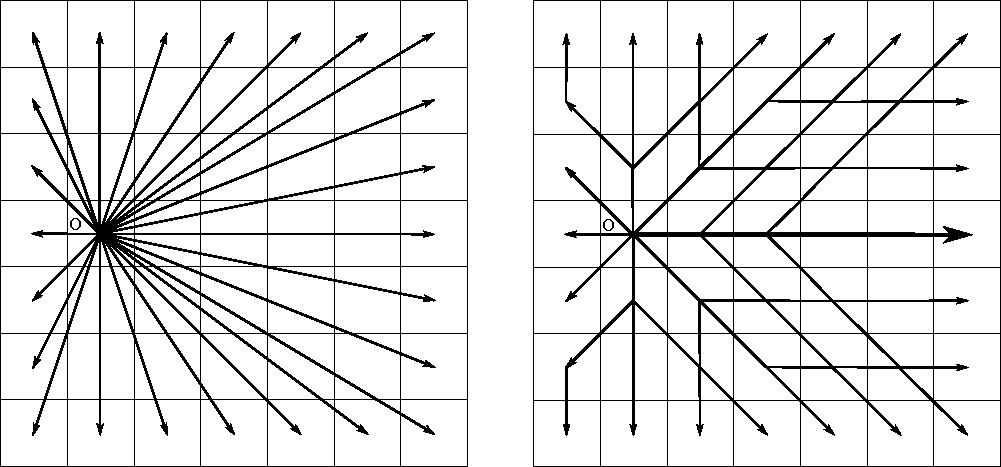
\includegraphics[scale=0.8]{img/grid.pdf} 
	\caption{Rayons lancés sur une image de 7x7 pixels à partir d'un point d'observation situé en (4,2). A gauche, le tracé théorique des rayons, à droite le parcours réel des rayons sur les pixels de l'image.}
	\label{grid}
\end{figure}

Pour chaque rayon, les pixels sont parcourus du plus proche du point O aux plus éloignés. A chaque pixel, l'angle de visé vertical entre le point O et le centre du pixel est calculé. Si l'angle est supérieur aux précédents, le pixel est visible, sinon il ne l'est pas. 

La hauteur des pixels correspond à la somme de l'altitude du MNT et de la hauteur du MNE s'il est présent. La hauteur du point d'observation O correspond à la somme de l'altitude du MNT et du paramètre h1 (Hauteur de l'oeil de l'observateur). La hauteur du MNE n'est jamais prise en compte pour la hauteur de l'observateur (l'observateur ne grimpe pas aux arbres).

La figure \ref{ray_side} représente le calcul d'un rayon sur 5 pixels. Le pixel situé sur le point de l'observateur (pixel 0) est toujours visible. Le pixel suivant (1) est aussi visible, par contre le pixel 2 ne l'est pas car l'angle de visé est plus faible que pour le pixel 1, et ainsi de suite.

\begin{figure}[H]
	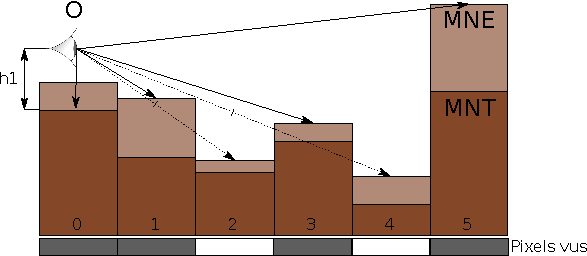
\includegraphics{img/ray_side-fr.pdf} 
	\caption{Vue de profil du lancer d'un rayon.}
	\label{ray_side}
\end{figure}

Le résultat du calcul du rayon de la figure \ref{ray_side} est montré sur la figure suivante (\ref{grid_result}). Il correspond aux pixels de l'image qui sont traversés par le rayon et qui sont visibles depuis le point d'observation.

\begin{figure}[H]
	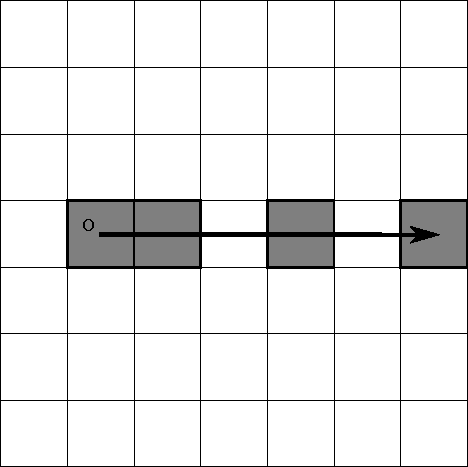
\includegraphics[scale=0.8]{img/grid_result.pdf} 
	\caption{Résultat en vue planimétrique du rayon calculé sur la figure \ref{ray_side}. Les pixels en gris sont les pixels visibles pour ce rayon.}
	\label{grid_result}
\end{figure}

Le résultat complet correspond à la combinaison des résultats pour chaque rayon.
Comme les pixels de l'image peuvent être traversés par des rayons différents, un pixel est marqué visible à partir du moment où il est visible par au moins un des rayons le traversant.

\subsection{Vue planimétrique inverse}

Le mode inverse permet d'inverser l'observateur et l'observé. Le bassin de visibilité n'est plus l'espace visible depuis le point O mais l'espace qui voit le point O. Le point O devient le point observé et l'observateur est positionné sur l'ensemble des points de l'image. La figure \ref{ray_side_inverse} montre le processus pour un rayon donné. 

\begin{figure}[H]
	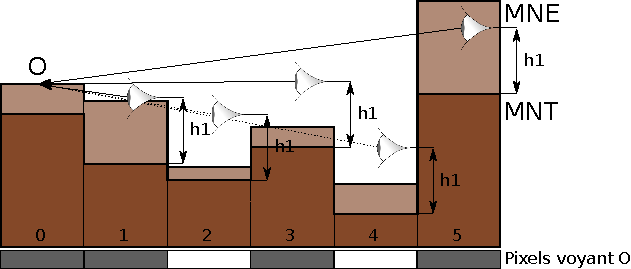
\includegraphics{img/ray_side_inverse-fr.pdf} 
	\caption{Vue de profil du lancer d'un rayon en mode inversé.}
	\label{ray_side_inverse}
\end{figure}

Le résultat est identique dans cet exemple, mais selon la configuration, il peut être différent en vue inverse.

\section{Vue tangentielle}
\label{principles_tan}
Pour la vue tangentielle, le principe de calcul est proche mais comporte quelques différences. Premièrement, le parcours de l'image n'est pas forcément exhaustif. Le nombre de rayons calculés n'est plus dépendant de la taille de l'image mais du paramètre de résolution angulaire $\alpha$. Par défaut, ce paramètre est défini à 0,1°. Le nombre de rayons calculés est de 3600. La figure \ref{grid_tan} montre un exemple avec une précision angulaire de 30°.

\begin{figure}[H]
	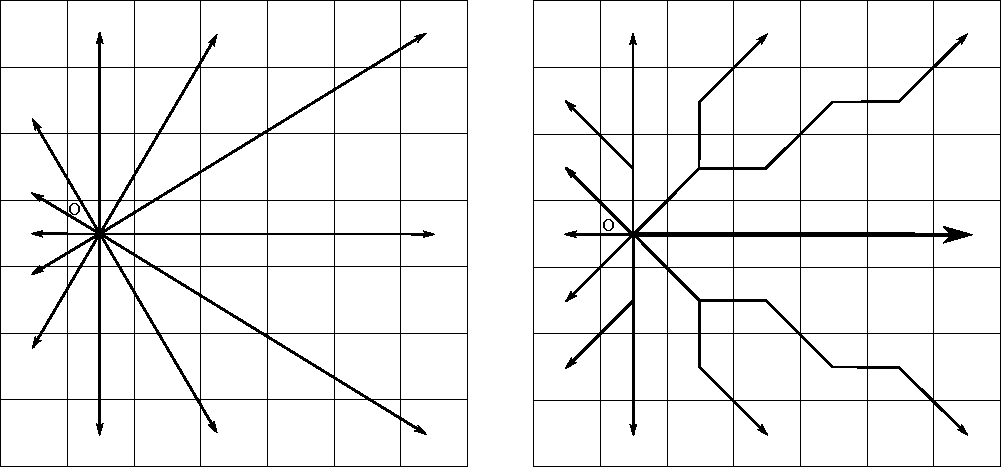
\includegraphics[scale=0.8]{img/grid_tan.pdf} 
	\caption{Rayons lancés sur une image de 7x7 pixels à partir d'un point d'observation situé en (4,2). A gauche, le tracé théorique des rayons, à droite le parcours réel des rayons sur les pixels de l'image. La précision angulaire ($\alpha$) est ici très grossière : 30°.}
	\label{grid_tan}
\end{figure}


Au niveau du calcul de chaque rayon, un traitement supplémentaire doit être réalisé pour déterminer la hauteur d'angle de chaque pixel visible (figure \ref{ray_side_tan}). Le résultat est représenté par la colonne à droite de la figure \ref{ray_side_tan} pour une précision angulaire ($\alpha$) de 10°.

\begin{figure}[H]
	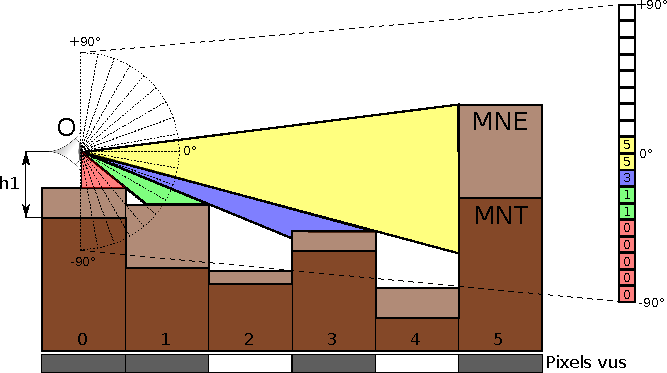
\includegraphics{img/ray_side_tan-fr.pdf} 
	\caption{Vue de profil du lancer d'un rayon. Calcul des hauteurs d'angle des pixels visibles pour la vue tangentielle. La précision angulaire est ici très grossière : 10°.}
	\label{ray_side_tan}
\end{figure}

La juxtaposition des colonnes résultant de chaque rayon forme le résultat de la vue tangentielle. La figure \ref{grid_tan_result} montre le positionnement de chaque rayon calculé dans la vue tangentielle pour une précision angulaire de 30°.

\begin{figure}[H]
	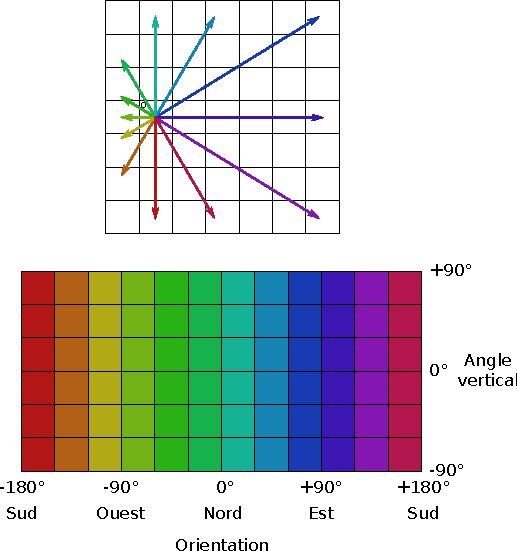
\includegraphics{img/grid_tan_result.pdf} 
	\caption{Position de chaque rayon dans la vue tangentielle résultante. La précision angulaire est ici très grossière : 30°.}
	\label{grid_tan_result}
\end{figure}

\section{Multi-résolution}
\label{multires}
Le calcul en multi-résolution permet d'accélérer fortement les traitements de visibilité. En effet, la complexité algorithmique d'un calcul de visibilité est proportionnel au nombre de pixels de l'image $n$. En multi-résolution, la complexité diminue à $log(n)$ du moment que les résolutions évoluent géométriquement.

\begin{figure}[H]
	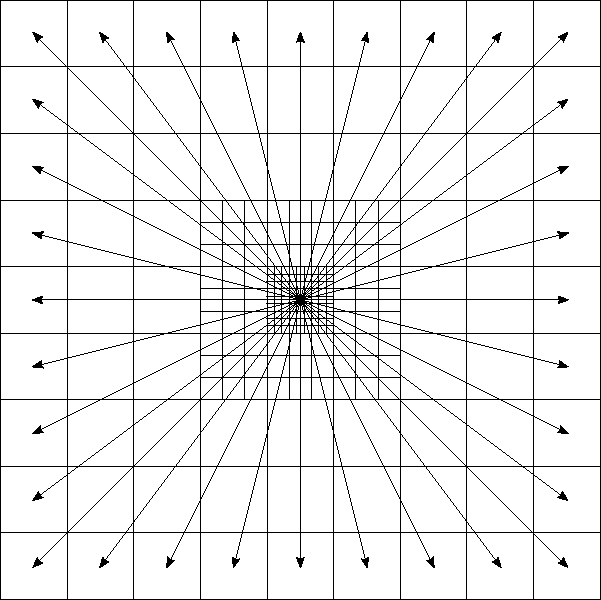
\includegraphics{img/grid_multi.pdf} 
	\caption{Rayons lancés sur une base multi-résolution d'un facteur 3 avec 3 résolutions}
	\label{grid_multi}
\end{figure}

Dans l'exemple de la figure \ref{grid_multi}, le nombre de rayons calculés est de 32 au lieu de 306 et la longueur des rayons en pixel est de 11 au lieu de 41. Le gain en temps de calcul est approximativement de 35 tout en conservant la contrainte de couverture complète de l'espace.


\section{Limitation du champ de vision}
\label{bounds}
Pour tous les calculs de visibilité intégrés dans PixScape, le champ de vision peut être restreint dans les 3 dimensions (figures \ref{bounds_side} et \ref{bounds_2d}) par 6 paramètres : la distance minimale ($d_{min}$) et maximale ($d_{max}$), l'angle vertical minimal ($z_{min}$) et maximal ($z_{max}$) et l'angle horizontal par l'orientation ($orien$) et l'amplitude ($amp$). Les angles sont exprimés en degré dans l'intervalle [0-360] pour les angles horizontaux et [-90;+90] pour les angles verticaux. Les distances sont exprimées en mètre et sont calculées en 2D sur le plan (x,y). 

\begin{figure}[H]
	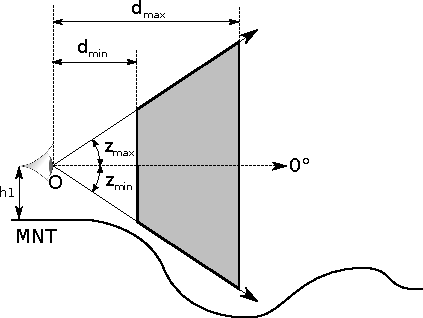
\includegraphics{img/bounds_side.pdf} 
	\caption{Vue de profil des limites du champ de vision}
	\label{bounds_side}
\end{figure}

\begin{figure}[H]
	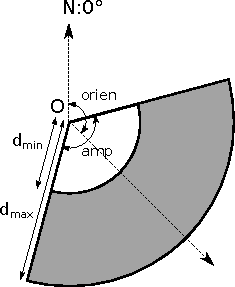
\includegraphics{img/bounds_2d.pdf} 
	\caption{Vue du dessus des limites du champ de vision}
	\label{bounds_2d}
\end{figure}


\chapter{Description des métriques}
\label{metrics}
Dans ce chapitre, l'ensemble des métriques disponibles dans PixScape sont décrites. Le tableau \ref{metrics_tab} liste l'ensemble de ces métriques et ce qu'elles supportent : support des vues planimétrique et/ou tangentielle, support ou non de l'occupation du sol et support des intervalles de distance.

\begin{table}[H]
	\begin{tabular}{|c|c|c|c|c|c|c|}
		\hline
		Métrique & Nom & Planimétrique & Tangentiel & Sans OS & Avec OS & Distance\\
		\hline
		A & Surface & X & X & X & X & X\\
		\hline
		S & Shannon OS & X & X &  & X & X\\
		\hline
		AG & Indice d'agrégation & X & X &  & X & \\
		\hline
		CONTAG & Contagion & X & X &  & X & \\
		\hline
		ED & Densité de bord & X & X &  & X & \\
		\hline
		PD & Densité de taches & X & X &  & X & \\
		\hline
		PMS & Taille moyenne des taches & X & X &  & X & \\
		\hline
		DIST & Distribution des distances & X & X & X &  & \\
		\hline
		P & Périmètre & X &  & X &  & \\
		\hline
		C & Compacité & X &  & X &  & \\
		\hline
		FD & Dimension fractale & X &  & X &  & \\
		\hline
		SL & Ligne d'horizon &  & X & X &  & X \\
		\hline
		SD & Shannon profondeur &  & X & X &  & \\
		\hline
		DL & Profondeur de vue &  & X & X &  & \\		
		\hline
	\end{tabular}
	\caption{Liste des métriques et de leur paramétrage}
	\label{metrics_tab}
\end{table}

\section{Métriques communes}

\subsection{Surface : A}
Cette métrique mesure la superficie visible en mètre carré pour la vue planimétrique et en degré carré pour la vue tangentielle. On peut restreindre le calcul à certaines catégories d'occupation du sol et pour différents intervalles de distance.


\subsection{Shannon OS : S}
Cette métrique calcule l'indice de Shannon sur les parts de surface visible de chaque catégorie d'occupation du sol.

$$S = -\frac{1}{\ln n}\sum_{i=1}^{n}\frac{A_i}{A}\ln\left(\frac{A_i}{A}\right)$$

Avec $n$ le nombre de catégories d'occupation du sol, $A_i$ la surface visible de la catégorie $i$ et $A$ la surface totale visible. L'unité des surfaces est en mètre carré pour la vue planimétrique et en degré carré pour la vue tangentielle.

Le projet doit contenir la couche d'occupation du sol pour pouvoir calculer cette métrique.

\subsection{Indice d'agrégation : AG}
Cette métrique correspond à "Aggregation Index" (AI) défini dans Fragstat. Dans PixScape, le calcul de cette métrique est appliquée uniquement aux surfaces d'occupation du sol visibles.

$$AG = \sum_{i=1}^n \frac{A_i}{A} AG_i, AG_i = 100 \frac{g_{ii}}{\max g_{ii}}$$

Avec $g_{ii}$ le nombre d'adjacence entre 2 pixels de la catégorie d'occupation du sol $i$ et $\max g_{ii}$ le maximum théorique \textit{ie.} quand la surface de la classe $i$ forme un carré.

Le projet doit contenir la couche d'occupation du sol pour pouvoir calculer cette métrique.

\subsection{Contagion : CONTAG}
Cette métrique correspond à l'indice "CONTAG" défini dans Fragstat. Dans PixScape, le calcul de cette métrique est appliquée uniquement aux surfaces d'occupation du sol visibles.

$$ CONTAG = 100 \left[1+\dfrac{1}{2\ln m} \sum _{i=1}^{m}  \sum _{j=1}^{m}  p_i\dfrac{g_{ij}}{\sum _{k=1}^{m}g_{ik} }   \ln \left( p_i\dfrac{g_{ij}}{\sum _{k=1}^{m}g_{ik} }\right)  \right]$$

Le projet doit contenir la couche d'occupation du sol pour pouvoir calculer cette métrique.

\subsection{Densité de bords : ED}
Cette métrique correspond à l'indice "Edge Density" (ED) défini dans Fragstat. Dans PixScape, le calcul de cette métrique est appliquée uniquement aux surfaces d'occupation du sol visibles.

$$ED = \frac{E}{A} = \frac{1}{2} \sum_{i=1}^{n} ED_i, ED_i = \frac{E_i}{A}$$

Avec $E$ le nombre d'adjacence entre 2 pixels de catégorie différente et $A$ la surface visible totale en mètre carré pour la vue planimétrique et en degré carré pour la vue tangentielle.

Les pixels au bord de la surface visible ne sont pas décomptés.

Le projet doit contenir la couche d'occupation du sol pour pouvoir calculer cette métrique.

\subsection{Densité de taches : PD}
Cette métrique correspond à l'indice "Patch Density" (PD) défini dans Fragstat. Dans PixScape, le calcul de cette métrique est appliquée uniquement aux surfaces d'occupation du sol visibles.

$$PD = \frac{p}{A} = \sum_{i=1}^{n} PD_i, PD_i = \frac{p_i}{A}$$

Avec $p_i$ le nombre de taches de la catégorie d'occupation du sol $i$ et $A$ la surface visible totale en mètre carré pour la vue planimétrique et en degré carré pour la vue tangentielle.

Le projet doit contenir la couche d'occupation du sol pour pouvoir calculer cette métrique.

\subsection{Taille moyenne des taches : PMS}
Cette métrique correspond à la taille moyenne des taches en mètre carré pour la vue planimétrique et en degré carré pour la vue tangentielle. Le calcul de cette métrique est appliquée uniquement aux surfaces d'occupation du sol visibles.

$$PMS = \frac{A}{p}, PMS_i = \frac{A_i}{p_i}$$

Avec $p_i$ le nombre de taches de la catégorie d'occupation du sol $i$ et $A$ la surface visible totale en mètre carré pour la vue planimétrique et en degré carré pour la vue tangentielle.

Le projet doit contenir la couche d'occupation du sol pour pouvoir calculer cette métrique.

\subsection{Distribution des distances : DIST}

La métrique $DIST$ donne un aperçu de la distribution des distances des pixels visibles depuis le point d'observation par quatre opérateurs d'agrégation : la somme, la moyenne, le minimum et le maximum.

Le résultat de la métrique est différent entre la vue tangentielle et planimétrique, les pixels visibles n'étant pas répartis de la même manière entre les deux vues. En effet, en planimétrique, chaque pixel représente une surface au sol en mètre carré, alors qu'en vue tangentielle, chaque pixel représente un cône du champ de vision en degré carré.


\section{Métriques planimétriques}

\subsection{Périmètre : P}

La métrique P correspond au périmètre total du bassin de visibilité, incluant l'ensemble des contours tant extérieur qu'intérieur. L'unité est en mètre.


\subsection{Compacité : C}
Cette métrique reprend l'indice de compacité appliqué au bassin de visibilité complet tel que :

$$C=\frac{P}{2\sqrt{\pi A}}$$

Si $C=1$ le bassin de visibilité est compact \textit{ie.} représente un disque plein. Plus $C$ augmente, moins le bassin de visibilité est compact.


\subsection{Dimension fractale : FD}
Cette métrique calcule la dimension fractale du bassin de visibilité. La méthode utilisée est le box counting.

Le résultat est compris entre 0 et 2. Quand $FD$ tend vers 0 le bassin se réduit à un point, quand $FD$ tend vers 2 le bassin couvre l'espace de façon homogène.

\section{Métriques tangentielles}

\subsection{Ligne d'horizon : SL}

La métrique $SL$ mesure l'aspect plus ou moins accidenté de la ligne d'horizon. Elle est calculée comme le rapport entre la longueur de la ligne d'horizon ($l_h$) et une ligne d'horizon plate ($L=360\deg$). Les longueurs sont exprimées en degré. 

$$SL=\frac{l_h}{L}$$

Quand $SL=1$ l'horizon est plat, plus $SL$ augmente plus la ligne d'horizon est accidentée.

\subsection{Shannon profondeur : SD}
La métrique $SD$ mesure la plus ou moins grande variation des profondeurs de vue.

Elle correspond à l’indice de Shannon standardisé appliqué à la distribution des profondeurs de vue regroupées en $m$ classes. Les classes de distance sont définies par une suite géométrique : inférieur à 10m, de 10 à 100m, de 100m à 1km, de 1km à 10km, et plus de 10km.

$$SD = -\frac{1}{\ln m}\sum_{i=1}^{m}\frac{nd_i}{n}\ln\left(\frac{nd_i}{n}\right)$$

avec $nd_i$ le nombre de longueurs maximales dans la classe de distance $i$ et $n$ le nombre total de rayons calculés dans la vue tangentielle.

Cette métrique vaut 0 quand toutes les longueurs sont dans la même classe et donc la profondeur de vue est homogène. A l’inverse, elle vaut 1 quand les longueurs de vue sont uniformément réparties dans toutes les classes, ce qui représente une grande variété de profondeurs de vue.

\subsection{Profondeur de vue : DL}
La métrique $DL$ mesure aussi la plus ou moins grande variation des profondeurs de vue mais sans à priori de classes de distance comme $SD$.

Cette métrique nécessite la construction d’un polygone sur le plan (x,y) regroupant les points visibles les plus éloignés du point d’observation pour chaque rayon lancé. La métrique $DL$ est définie comme l’indice de compacité de ce polygone : 

$$DL=\frac{p}{2\sqrt{\pi a}}$$

où $p$ et $a$ représentent respectivement le périmètre et l’aire du polygone. 

Cette métrique donne une valeur minimale de 1 dans le cas de profondeurs de vue égales (le polygone forme un cercle), et des valeurs élevées (non bornées) dans le cas de variations fortes des profondeurs de vue.


\chapter{Performances}
\label{perf}

\section{Parallélisation}
\label{parallelism}
Pour diminuer les temps d'exécution de calcul de visibilité, PixScape implémente 3 méthodes de parallélisation : par thread pour un ordinateur seul, par CUDA pour utiliser l'accélération GPU (Graphics Processor Unit) et par MPI pour les clusters d'ordinateurs.

Le tableau \ref{perf_table} montre les temps d'exécution pour calculer 10000 vues selon le type de vue (planimétrique ou tangentiel), la taille du MNT en million de pixels et la parallélisation : 1 coeur (sans parallélisation), 4 coeurs, 16 coeurs et GPU (carte graphique NVidia Tesla K40).

\begin{table}[htbp]
	
	\begin{tabular}{|l|r|r|r|r|r|}
		\hline
		Type & \multicolumn{1}{l|}{Taille} & \multicolumn{1}{l|}{1 coeur} & \multicolumn{1}{l|}{4 coeurs} & \multicolumn{1}{l|}{16 coeurs} & \multicolumn{1}{l|}{GPU} \\ \hline
		\multicolumn{ 1}{|c|}{Planimétrique} & 1 M & 9,8 & 2,5 & 0,7 & 0,6 \\ \cline{ 2- 6}
		\multicolumn{ 1}{|l|}{} & 9 M & 103,0 & 26,0 & 6,7 & 1,8 \\ \cline{ 2- 6}
		\multicolumn{ 1}{|l|}{} & 100 M & 1168,0 & 376,0 & 83,0 & 13,2 \\ \hline
		\multicolumn{ 1}{|c|}{Tangentiel} & 1 M & 36,0 & 9,8 & 2,7 & 0,8 \\ \cline{ 2- 6}
		\multicolumn{ 1}{|l|}{} & 9 M & 113,0 & 28,8 & 8,0 & 2,2 \\ \cline{ 2- 6}
		\multicolumn{ 1}{|l|}{} & 100 M & 357,0 & 91,0 & 24,7 & 6,3 \\ \hline
	\end{tabular}
	\caption{Temps moyen en minute pour calculer 10000 vues.}
	\label{perf_table}
\end{table}



\subsection{Un ordinateur : threads}
\label{thread}
La parallélisation par thread accélère le calcul sur une seule machine contenant plusieurs cœurs ou processeurs.
Si votre ordinateur a plus qu'un coeur (la plupart), vous pouvez tirer partie de la parallélisation par thread pour accélérer vos calculs avec PixScape. Le temps d'exécution est approximativement inversement proportionnel au nombre de coeurs utilisés. Ce mode de parallélisation est utilisable en interface graphique et en ligne de commande.

\subsubsection{Interface graphique}
La fenêtre "Préferences" accessible par le menu Fichier permet de régler le nombre de coeurs utilisés par PixScape. Il est défini par défaut au nombre coeurs de la machine moins 1. Après avoir modifié le nombre de coeurs utilisé par PixScape, il vaut mieux relancer PixScape pour être sûr que le changement soit bien pris en compte.

\subsubsection{Ligne de commande}
En ligne de commande, il faut définir le nombre de coeurs (ou processeurs) que PixScape peut utiliser avec l'option \verb|-proc| :
\begin{Verbatim}
	java -jar pixscape-1.0.jar -proc 8 --project path2myproject/myproject.xml ...
\end{Verbatim}
Par défaut, en ligne de commande, le nombre de coeurs utilisés correspond au nombre défini dans la fenêtre Préférences de l'interface graphique.

En augmentant le nombre de coeurs utilisés par PixScape, vous augmentez, par la même occasion, la taille de la mémoire utilisée par PixScape.

\subsection{Carte graphique : CUDA}
\label{cuda}
Ce mode de parallélisation permet de réaliser les calculs de visibilité sur la carte graphique au lieu du processeur. Les gains en temps d'exécution peuvent être important pour des cartes graphiques Nvidia de la gamme Tesla, conçues pour le calcul haute performance (voir \nameref{perf_table}). Par contre toutes les métriques ne sont pas optimisées pour le GPU. Les métriques A et S sont les seules à être optimisées. Si vous utilisez d'autres métriques, les gains de temps seront minimes voire inexistant.

Pour pouvoir utiliser l'accélération GPU il faut une carte graphique Nvidia supportant CUDA et que la version 6.5 de CUDA soit installée. 

Si PixScape n'arrive pas à utiliser le GPU, les calculs seront basculés automatiquement sur le processeur.

Ce mode de parallélisation est utilisable en interface graphique et en ligne de commande.

\subsubsection{Interface graphique}

L'activation de l'accélération GPU est accessible à partir de la fenêtre Options (voir \nameref{options}).

En interface graphique, PixScape ne peut utiliser qu'une seule carte graphique, si votre ordinateur contient plusieurs cartes graphiques, PixScape peut les utiliser en parallèle mais uniquement en ligne de commande.

\subsubsection{Ligne de commande}
En ligne de commande, l'option \verb|-cuda| permet d'activer l'utilisation du GPU. Il faut aussi donner le nombre de cartes graphiques à utiliser.

\begin{Verbatim}
	java -jar pixscape-1.0.jar -cuda 1 --project path2myproject/myproject.xml ...
\end{Verbatim}
Dans l'exemple ci-dessus, PixScape utilisera une carte graphique pour les calculs de visibilité. Si votre ordinateur contient plusieurs cartes graphiques il est possible d'augmenter le paramètre pour les utiliser en parallèle et diminuer d'autant le temps d'exécution.


\subsection{Cluster : MPI}
PixScape peut aussi être utilisé sur des clusters de calcul supportant Java avec OpenMPI. Ce mode de parallélisation n'est accessible qu'en ligne de commande.

Exemple :
\begin{Verbatim}
	mpirun java -jar pixscape-1.0.jar -mpi --project path2myproject/myproject.xml ...
\end{Verbatim}
Seulement certaines commandes peuvent être utilisées dans l'environnement MPI : \verb|--planmetric|, \verb|--tanmetric|, \verb|--landmod|


\section{Gestion mémoire}
\label{memory}
Par défaut, la taille de la mémoire utilisable par PixScape est dépendante du système et peut varier de 128 MB à plusieurs GB.
Si vous avez un gros projets, certaines commandes stopperont le programme à cause d'un manque de mémoire. De plus, si vous utilisez la parallélisation par thread (\nameref{thread}), PixScape aura besoin de plus de mémoire pour chaque coeur utilisé.
Dans tous les cas, si l'exécution se termine par une erreur OutOfMemoryError ou GC overhead, vous devez augmenter la mémoire disponible pour PixScape.

\subsection{Interface graphique}
La mémoire allouée pour PixScape peut être modifiée dans la fenêtre "Préférences" dans le menu Fichier / Préférences. Après avoir changé ce paramètre, PixScape doit être relancé pour qu'il tienne compte de la nouvelle taille mémoire.

En interface graphique, PixScape a besoin de plus de mémoire qu'en ligne de commande du fait de l'affichage des couches. Si vous êtes trop limité en mémoire vive, vous pouvez lancer les calculs en ligne de commande pour diminuer les besoins en mémoire de PixScape (voir \nameref{cli}).

\subsection{Interface en ligne de commande}
Pour définir la mémoire maximale utilisable par PixScape en ligne de commande, il faut utiliser l'option Java \verb|-Xmx| :
\begin{Verbatim}
	java -Xmx4g -jar pixscape-1.0.jar ... # 4Gb allocated
	java -Xmx1500m -jar pixscape-1.0.jar ... # 1500 Mb -> 1.5Gb allocated
\end{Verbatim}


Si vous ne pouvez pas allouer plus de 1 GB ou 1.5 GB alors que votre ordinateur a plus de mémoire vive, vous utilisez sûrement une version 32-bit de Java qui est limitée à moins de 2 GB.
Pour tester votre version de Java :
\begin{Verbatim}
	java -version
\end{Verbatim}
Si vous avez une version 32-bit, installez une version 64-bit de Java pour allouer plus de mémoire à PixScape.


%\section{Multi-résolution}

\end{document}
